% Options for packages loaded elsewhere
\PassOptionsToPackage{unicode}{hyperref}
\PassOptionsToPackage{hyphens}{url}
\PassOptionsToPackage{dvipsnames,svgnames,x11names}{xcolor}
%
\documentclass[
  letterpaper,
  DIV=11,
  numbers=noendperiod]{scrartcl}

\usepackage{amsmath,amssymb}
\usepackage{iftex}
\ifPDFTeX
  \usepackage[T1]{fontenc}
  \usepackage[utf8]{inputenc}
  \usepackage{textcomp} % provide euro and other symbols
\else % if luatex or xetex
  \usepackage{unicode-math}
  \defaultfontfeatures{Scale=MatchLowercase}
  \defaultfontfeatures[\rmfamily]{Ligatures=TeX,Scale=1}
\fi
\usepackage{lmodern}
\ifPDFTeX\else  
    % xetex/luatex font selection
\fi
% Use upquote if available, for straight quotes in verbatim environments
\IfFileExists{upquote.sty}{\usepackage{upquote}}{}
\IfFileExists{microtype.sty}{% use microtype if available
  \usepackage[]{microtype}
  \UseMicrotypeSet[protrusion]{basicmath} % disable protrusion for tt fonts
}{}
\makeatletter
\@ifundefined{KOMAClassName}{% if non-KOMA class
  \IfFileExists{parskip.sty}{%
    \usepackage{parskip}
  }{% else
    \setlength{\parindent}{0pt}
    \setlength{\parskip}{6pt plus 2pt minus 1pt}}
}{% if KOMA class
  \KOMAoptions{parskip=half}}
\makeatother
\usepackage{xcolor}
\usepackage[top=20mm,left=20mm,right=20mm,bottom=20mm]{geometry}
\setlength{\emergencystretch}{3em} % prevent overfull lines
\setcounter{secnumdepth}{5}
% Make \paragraph and \subparagraph free-standing
\makeatletter
\ifx\paragraph\undefined\else
  \let\oldparagraph\paragraph
  \renewcommand{\paragraph}{
    \@ifstar
      \xxxParagraphStar
      \xxxParagraphNoStar
  }
  \newcommand{\xxxParagraphStar}[1]{\oldparagraph*{#1}\mbox{}}
  \newcommand{\xxxParagraphNoStar}[1]{\oldparagraph{#1}\mbox{}}
\fi
\ifx\subparagraph\undefined\else
  \let\oldsubparagraph\subparagraph
  \renewcommand{\subparagraph}{
    \@ifstar
      \xxxSubParagraphStar
      \xxxSubParagraphNoStar
  }
  \newcommand{\xxxSubParagraphStar}[1]{\oldsubparagraph*{#1}\mbox{}}
  \newcommand{\xxxSubParagraphNoStar}[1]{\oldsubparagraph{#1}\mbox{}}
\fi
\makeatother


\providecommand{\tightlist}{%
  \setlength{\itemsep}{0pt}\setlength{\parskip}{0pt}}\usepackage{longtable,booktabs,array}
\usepackage{calc} % for calculating minipage widths
% Correct order of tables after \paragraph or \subparagraph
\usepackage{etoolbox}
\makeatletter
\patchcmd\longtable{\par}{\if@noskipsec\mbox{}\fi\par}{}{}
\makeatother
% Allow footnotes in longtable head/foot
\IfFileExists{footnotehyper.sty}{\usepackage{footnotehyper}}{\usepackage{footnote}}
\makesavenoteenv{longtable}
\usepackage{graphicx}
\makeatletter
\def\maxwidth{\ifdim\Gin@nat@width>\linewidth\linewidth\else\Gin@nat@width\fi}
\def\maxheight{\ifdim\Gin@nat@height>\textheight\textheight\else\Gin@nat@height\fi}
\makeatother
% Scale images if necessary, so that they will not overflow the page
% margins by default, and it is still possible to overwrite the defaults
% using explicit options in \includegraphics[width, height, ...]{}
\setkeys{Gin}{width=\maxwidth,height=\maxheight,keepaspectratio}
% Set default figure placement to htbp
\makeatletter
\def\fps@figure{htbp}
\makeatother

\KOMAoption{captions}{tableheading}
\usepackage{sansmathfonts}
\usepackage[utf8]{inputenc}
\usepackage[T1]{fontenc}
\renewcommand*\familydefault{\sfdefault}
\makeatletter
\@ifpackageloaded{tcolorbox}{}{\usepackage[skins,breakable]{tcolorbox}}
\@ifpackageloaded{fontawesome5}{}{\usepackage{fontawesome5}}
\definecolor{quarto-callout-color}{HTML}{909090}
\definecolor{quarto-callout-note-color}{HTML}{0758E5}
\definecolor{quarto-callout-important-color}{HTML}{CC1914}
\definecolor{quarto-callout-warning-color}{HTML}{EB9113}
\definecolor{quarto-callout-tip-color}{HTML}{00A047}
\definecolor{quarto-callout-caution-color}{HTML}{FC5300}
\definecolor{quarto-callout-color-frame}{HTML}{acacac}
\definecolor{quarto-callout-note-color-frame}{HTML}{4582ec}
\definecolor{quarto-callout-important-color-frame}{HTML}{d9534f}
\definecolor{quarto-callout-warning-color-frame}{HTML}{f0ad4e}
\definecolor{quarto-callout-tip-color-frame}{HTML}{02b875}
\definecolor{quarto-callout-caution-color-frame}{HTML}{fd7e14}
\makeatother
\makeatletter
\@ifpackageloaded{caption}{}{\usepackage{caption}}
\AtBeginDocument{%
\ifdefined\contentsname
  \renewcommand*\contentsname{Table des matières}
\else
  \newcommand\contentsname{Table des matières}
\fi
\ifdefined\listfigurename
  \renewcommand*\listfigurename{Liste des Figures}
\else
  \newcommand\listfigurename{Liste des Figures}
\fi
\ifdefined\listtablename
  \renewcommand*\listtablename{Liste des Tables}
\else
  \newcommand\listtablename{Liste des Tables}
\fi
\ifdefined\figurename
  \renewcommand*\figurename{Figure}
\else
  \newcommand\figurename{Figure}
\fi
\ifdefined\tablename
  \renewcommand*\tablename{Table}
\else
  \newcommand\tablename{Table}
\fi
}
\@ifpackageloaded{float}{}{\usepackage{float}}
\floatstyle{ruled}
\@ifundefined{c@chapter}{\newfloat{codelisting}{h}{lop}}{\newfloat{codelisting}{h}{lop}[chapter]}
\floatname{codelisting}{Listing}
\newcommand*\listoflistings{\listof{codelisting}{Liste des Listings}}
\usepackage{amsthm}
\theoremstyle{definition}
\newtheorem{exercise}{Exercice}[section]
\theoremstyle{definition}
\newtheorem{definition}{Définition}[section]
\theoremstyle{definition}
\newtheorem{example}{Exemple}[section]
\theoremstyle{remark}
\AtBeginDocument{\renewcommand*{\proofname}{Preuve}}
\newtheorem*{remark}{Remarque}
\newtheorem*{solution}{Solution}
\newtheorem{refremark}{Remarque}[section]
\newtheorem{refsolution}{Solution}[section]
\makeatother
\makeatletter
\makeatother
\makeatletter
\@ifpackageloaded{caption}{}{\usepackage{caption}}
\@ifpackageloaded{subcaption}{}{\usepackage{subcaption}}
\makeatother

\ifLuaTeX
\usepackage[bidi=basic]{babel}
\else
\usepackage[bidi=default]{babel}
\fi
\babelprovide[main,import]{french}
% get rid of language-specific shorthands (see #6817):
\let\LanguageShortHands\languageshorthands
\def\languageshorthands#1{}
\ifLuaTeX
  \usepackage{selnolig}  % disable illegal ligatures
\fi
\usepackage{bookmark}

\IfFileExists{xurl.sty}{\usepackage{xurl}}{} % add URL line breaks if available
\urlstyle{same} % disable monospaced font for URLs
\hypersetup{
  pdftitle={La gravitation universelle},
  pdflang={fr},
  colorlinks=true,
  linkcolor={blue},
  filecolor={Maroon},
  citecolor={Blue},
  urlcolor={Blue},
  pdfcreator={LaTeX via pandoc}}


\title{La gravitation universelle}
\author{}
\date{}

\begin{document}
\maketitle


\begin{titlepage}
    \centering
    
    % Espace au-dessus du titre
    \vspace*{2cm} 
    
    % Titre principal en grand
    {\fontsize{24pt}{28pt}\selectfont\textbf{La loi de la gravitation universelle}\par}
    
    % Espace entre le titre et l'image
    \vspace*{1cm} 
    
    % Insertion de l'image
    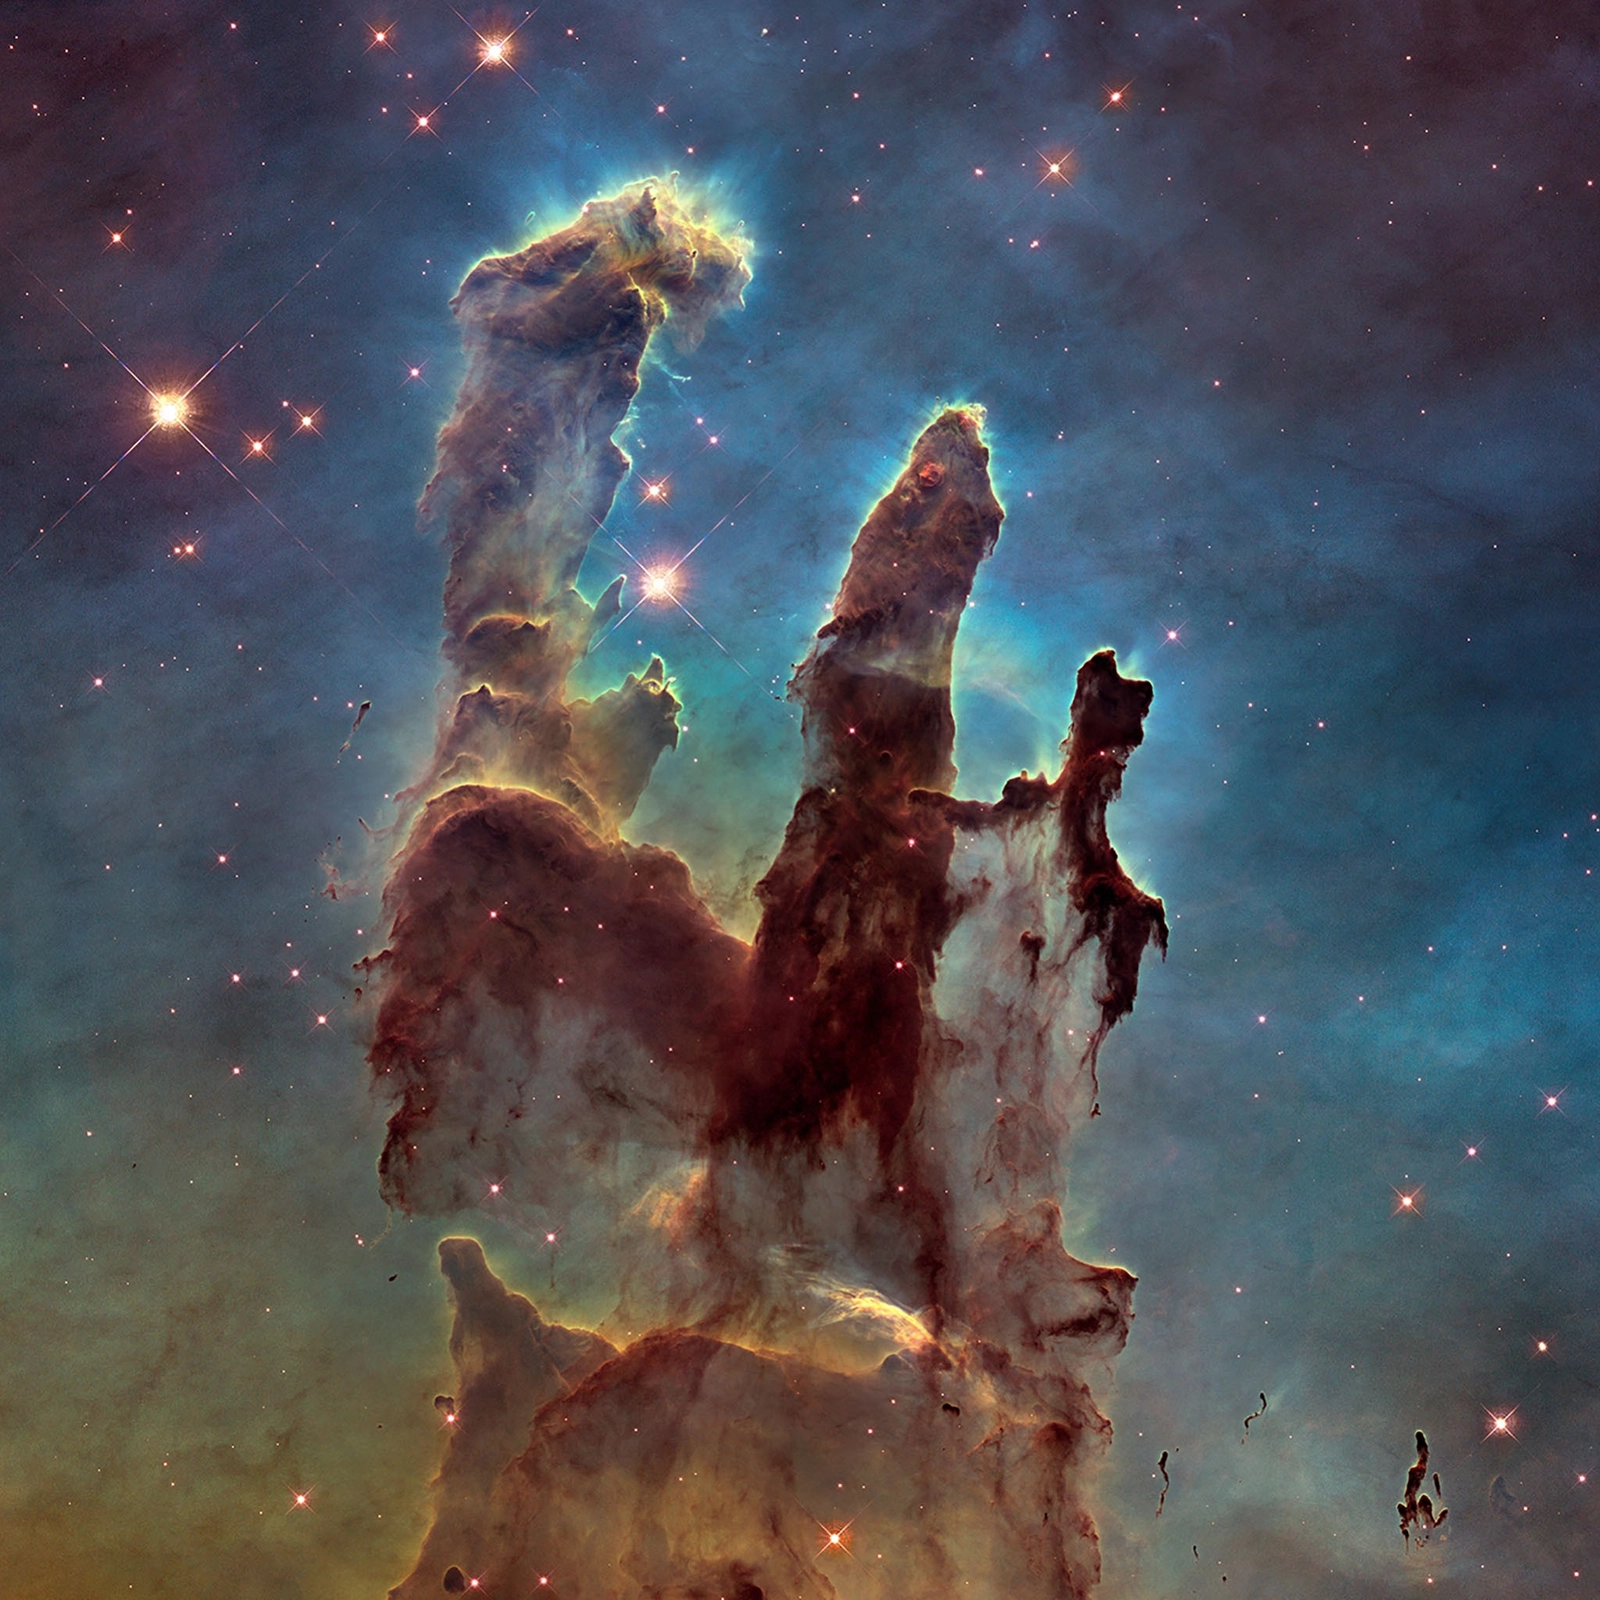
\includegraphics[width=\textwidth]{./figures/grav/nebula.png} % Ajustez width selon vos besoins
    

    
    % Espacement pour aligner le bas
    \vfill
    
\end{titlepage}

\section{Introduction: une longue histoire en quatre
étapes}\label{introduction-une-longue-histoire-en-quatre-uxe9tapes}

L'observation et l'étude des corps célestes est à l'origine de la loi de
la gravitation universelle.

\begin{figure}[H]

{\centering 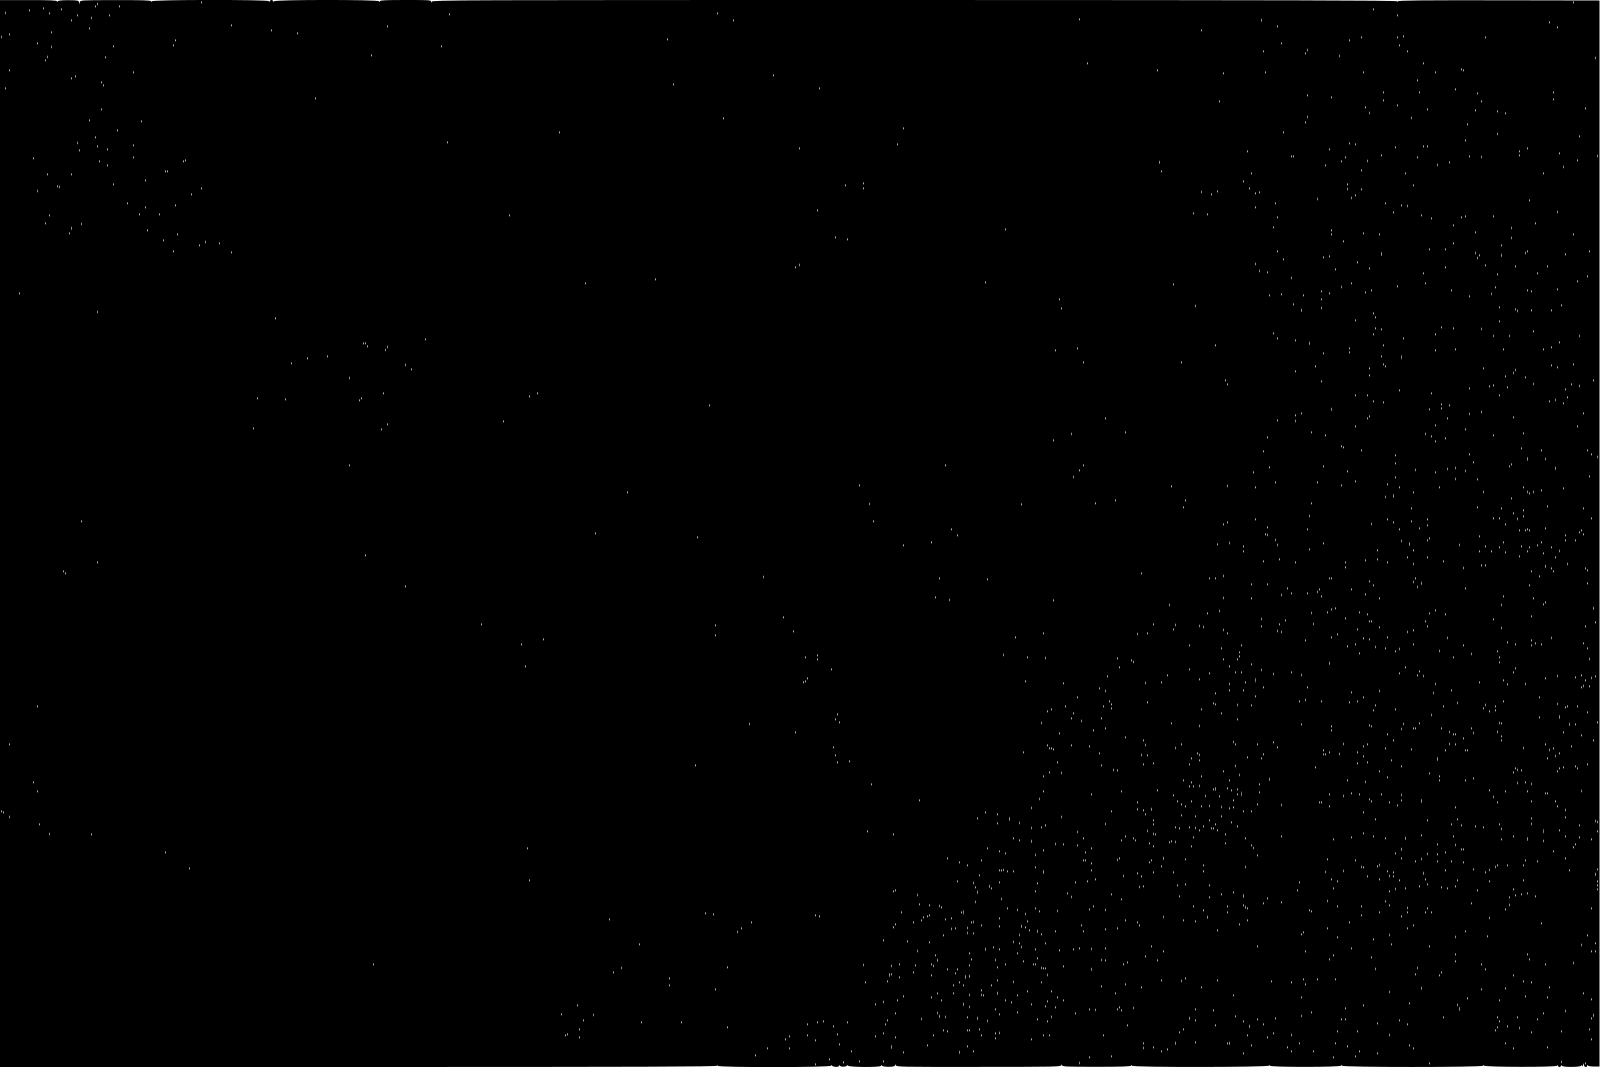
\includegraphics{figures/grav/01-milky-way-NationalGeographic_1959323.pdf}

}

\caption{La Voie Lactée}

\end{figure}%

\subsection{Les modèles
géocentriques}\label{les-moduxe8les-guxe9ocentriques}

Dès l'Antiquité, les savants ont observé les étoiles et ont essayé de
comprendre leur mouvement.

\begin{figure}[H]

{\centering 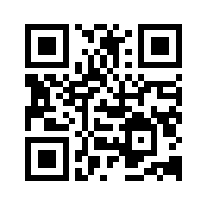
\includegraphics[width=0.2\textwidth,height=\textheight]{figures/grav/stell.pdf}

}

\caption{QR-code de l'application}

\end{figure}%

Les premiers modèles qui ont tenté de rendre compte du mouvement des
astres étaient géocentriques : le mouvement des astres se fait par
rotation autour de la Terre, qui est le centre de l'univers.

\begin{figure}[H]

{\centering 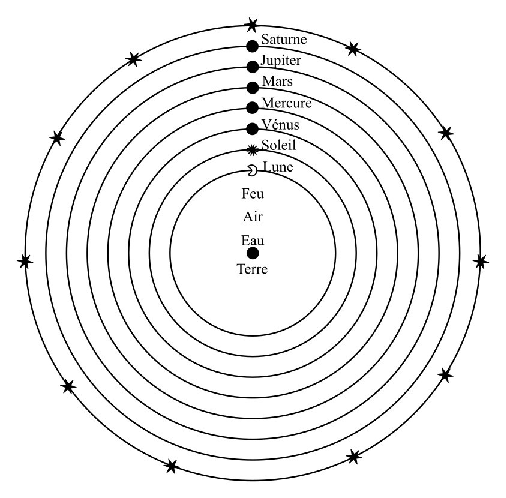
\includegraphics[width=0.4\textwidth,height=\textheight]{figures/grav/geo.pdf}

}

\caption{Le modèle géocentrique}

\end{figure}%

Cependant, ce modèle est très vite confronté à certaines difficultés.
L'une d'elles concerne le mouvement de Mars autour de la Terre.

\begin{figure}[H]

{\centering 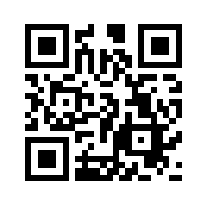
\includegraphics[width=0.2\textwidth,height=\textheight]{figures/grav/mars.pdf}

}

\caption{QR-code: Orbite de Mars autour de la Terre}

\end{figure}%

Tu peux observer sur l'animation ci-dessus que Mars a un mouvement
rétrograde autour de la Terre. Cette observation était déjà réalisée
plus de deux siècles avant Jésus-Christ, et deux savants de l'époque,
Apollonius et Hipparque, ont tenté d'expliquer pourquoi Mars a un tel
mouvement : ils ont mis au point les premiers modèles par épicycles. Ces
modèles décrivent le mouvement de Mars (mais aussi d'autres astres) de
la manière suivante : Mars se déplace le long d'un cercle, à vitesse
constante, et le centre de ce cercle se déplace lui-même sur un grand
cercle dont le centre est la Terre.

\begin{figure}[H]

{\centering 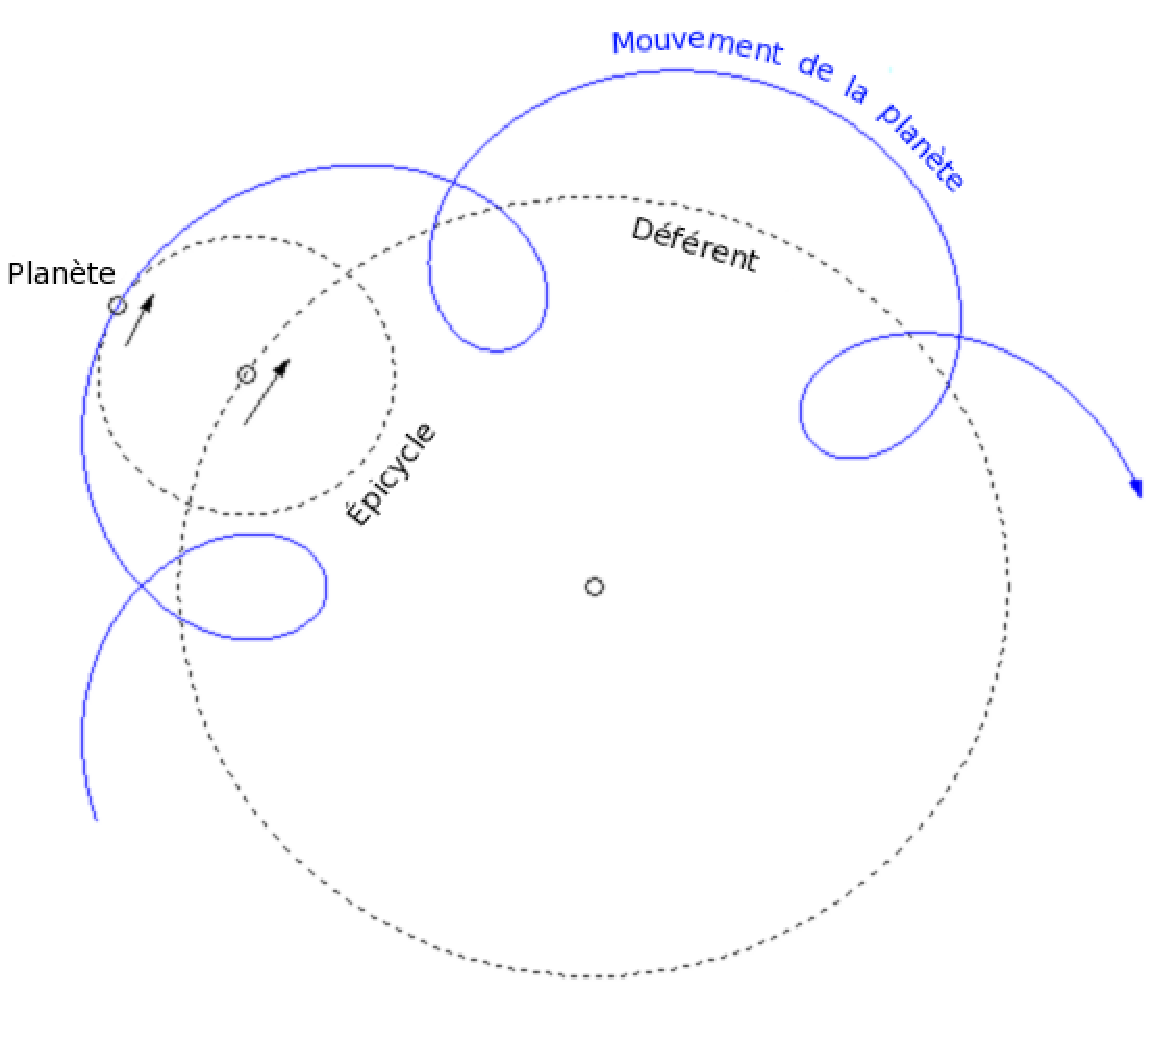
\includegraphics[width=0.4\textwidth,height=\textheight]{figures/grav/epicycle.pdf}

}

\caption{Modèle géocentrique avec épicycle}

\end{figure}%

Ces modèles par épicycles ont été étudiés et raffinés pendant longtemps,
pour aboutir au modèle de Ptolémée, qui proposa un modèle avec plusieurs
épicycles pour expliquer les défauts de mesure des modèles d'Apollonius
et Hipparque. Les travaux de Ptolémée furent la référence en astronomie
jusqu'au XVIe siècle, avec l'arrivée du modèle héliocentrique de
Copernic.

\subsection{Les modèles
héliocentriques}\label{les-moduxe8les-huxe9liocentriques}

Malgré la précision importante des modèles géocentriques, les astronomes
du XVIe siècle n'arrivent pas à prévoir parfaitement le mouvement des
astres. Copernic émit l'hypothèse que le Soleil était au centre de
l'Univers et que la Terre effectue un mouvement circulaire autour de lui
: c'est la naissance des modèles héliocentriques. Bien que le modèle
héliocentrique de Copernic représente une révolution en astronomie, il
ne permet pas une plus grande précision dans les prédictions que dans le
modèle de Ptolémée. La raison est que Copernic suppose que les astres
décrivent des cercles autour du Soleil.

\begin{figure}[H]

{\centering 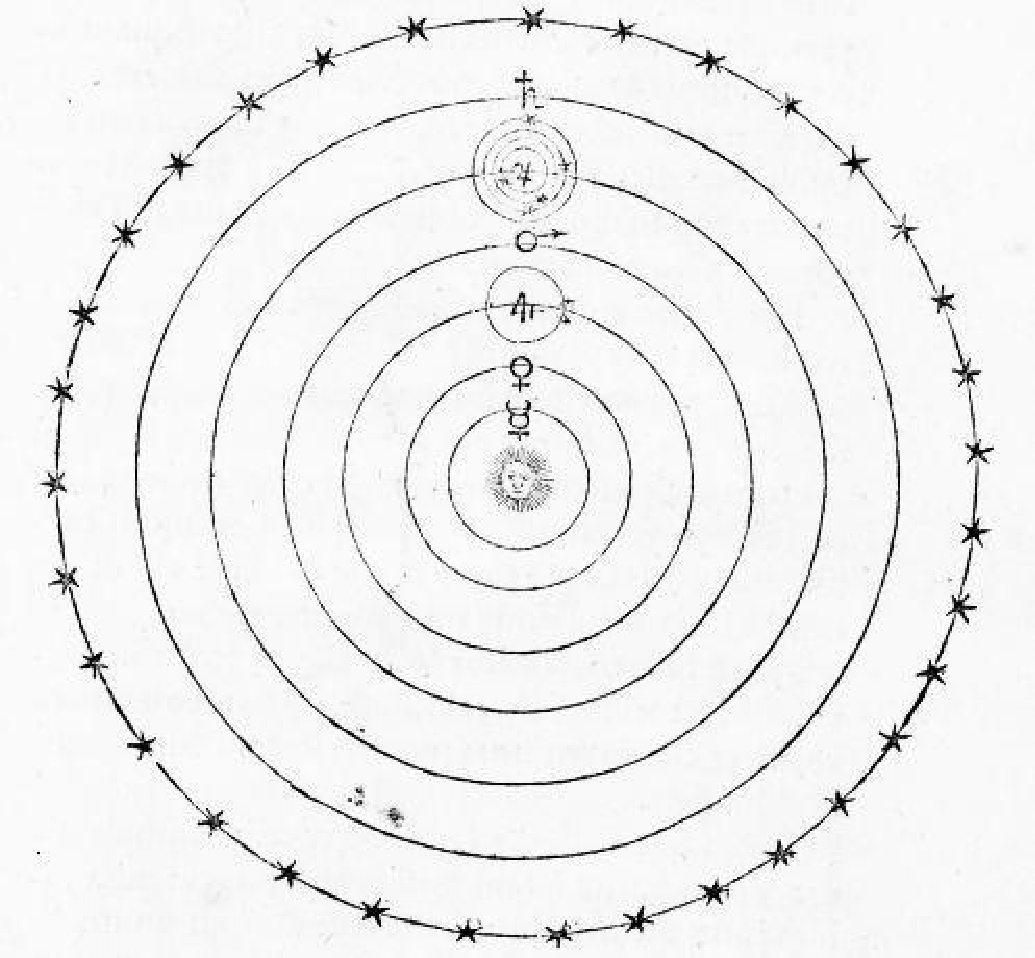
\includegraphics[width=0.4\textwidth,height=\textheight]{figures/grav/copernic.pdf}

}

\caption{Le modèle de Copernic}

\end{figure}%

Cependant, un atout du modèle de Copernic est sa simplicité par rapport
au modèle avec épicycles. De plus, le mouvement rétrograde de Mars
s'explique facilement comme un effet de perspective d'un observateur sur
Terre.

\begin{figure}[H]

{\centering 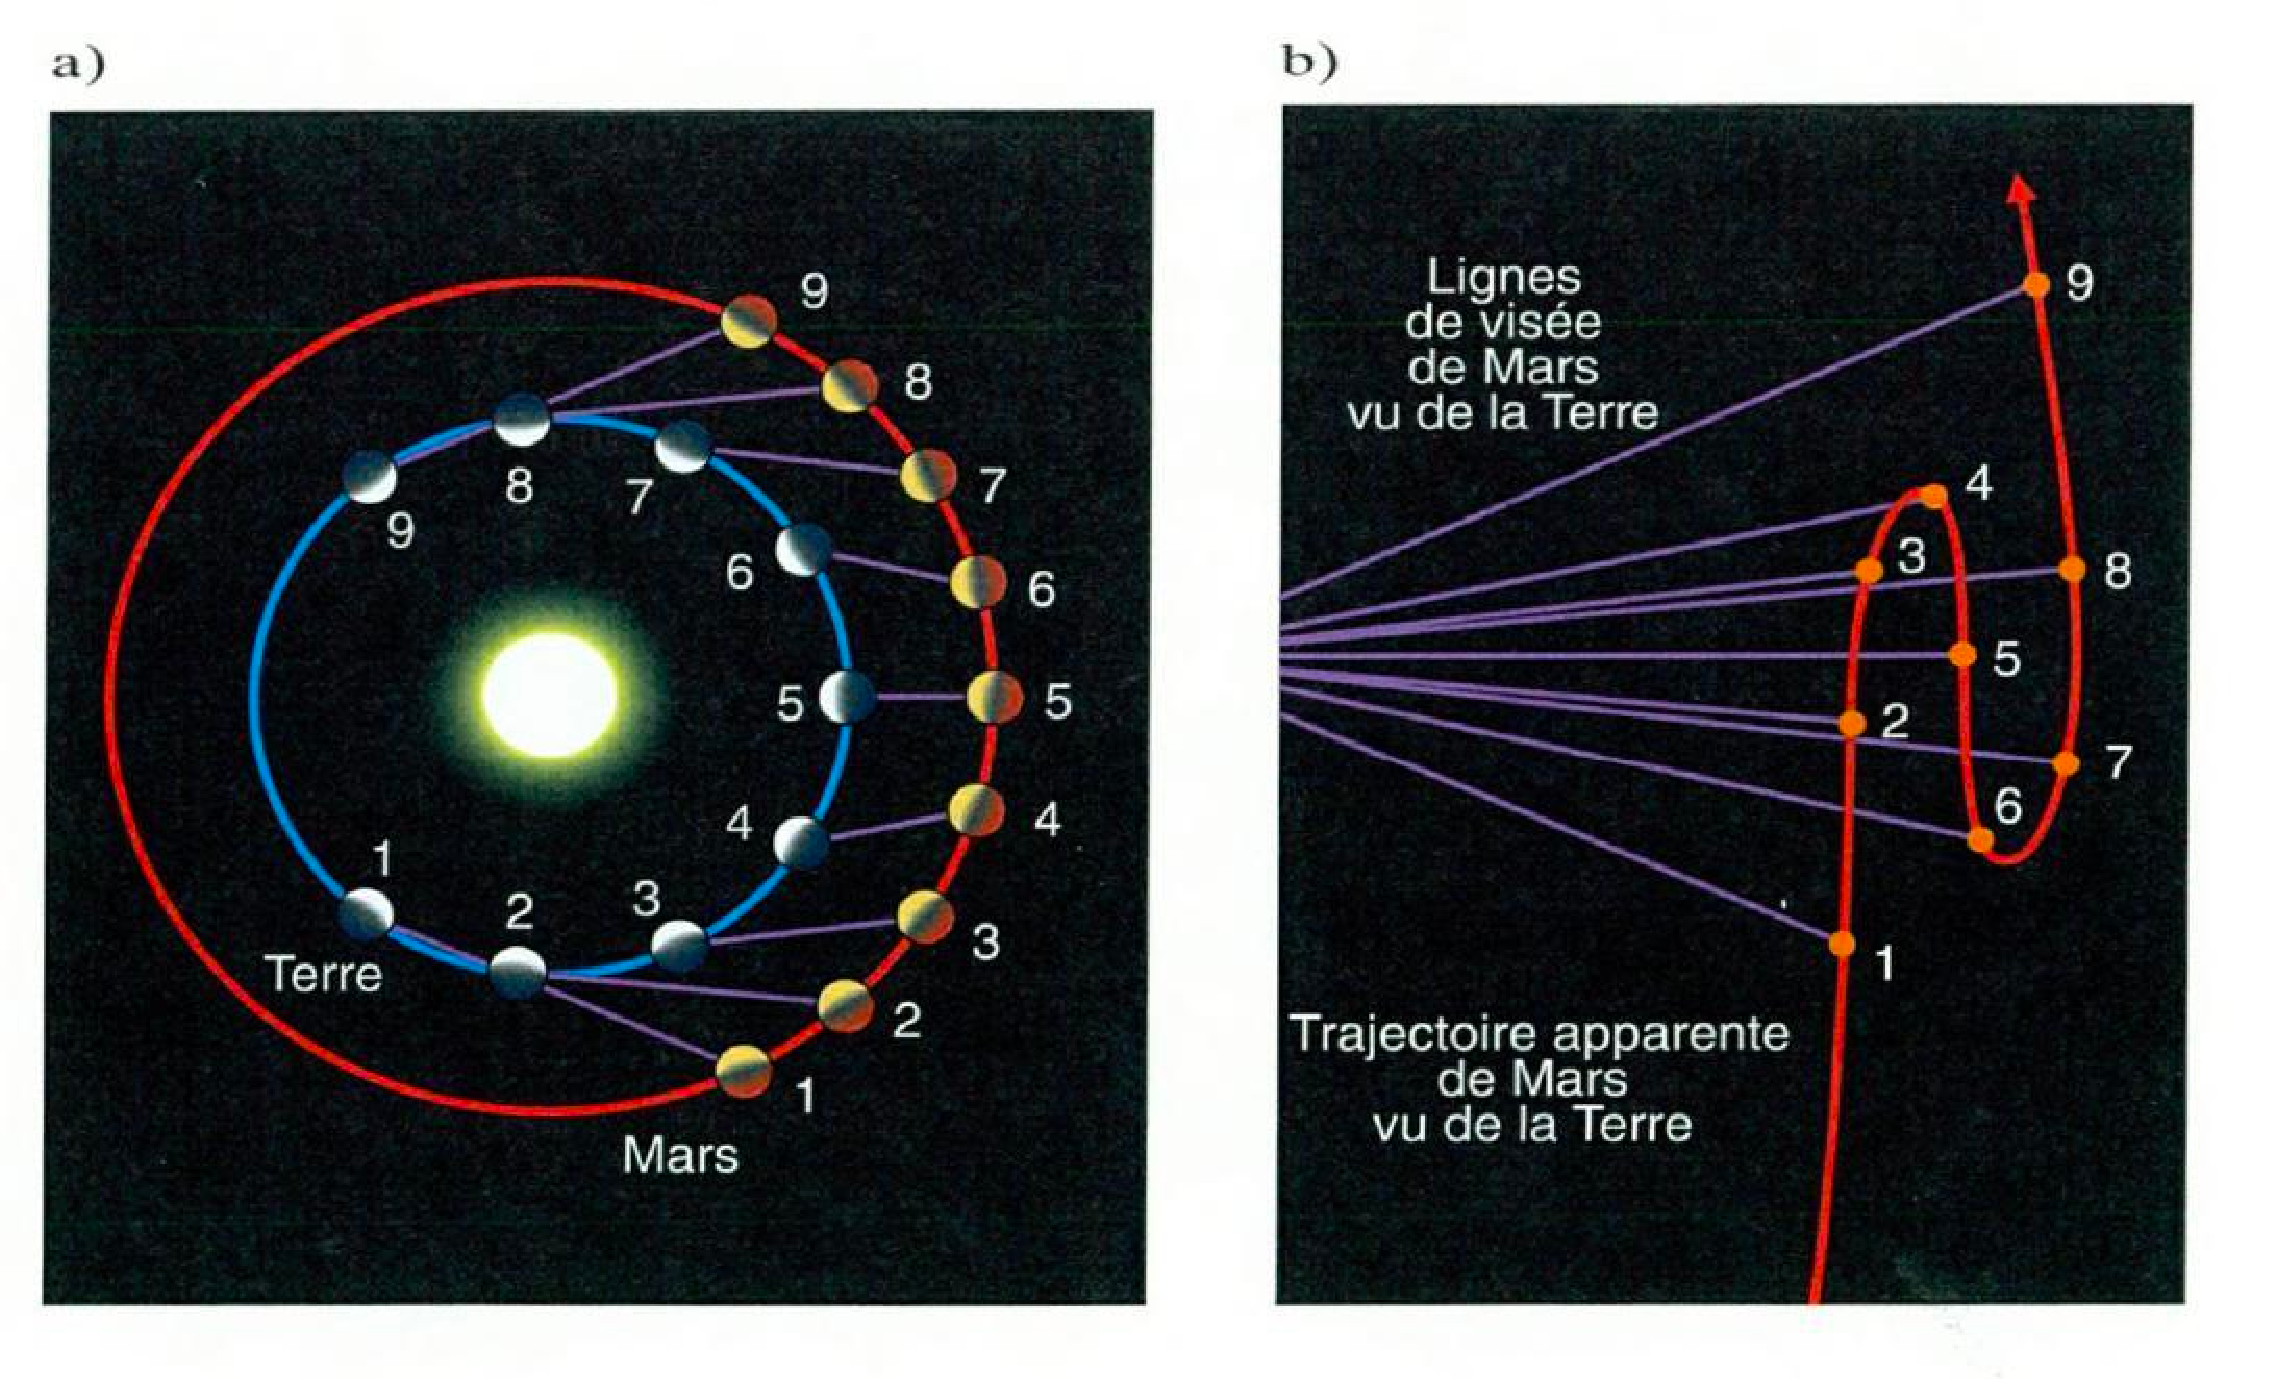
\includegraphics[width=1\textwidth,height=\textheight]{figures/grav/mars-2.pdf}

}

\caption{Orbite de Mars dans le modèle héliocentrique}

\end{figure}%

Le modèle de Copernic ne rencontrera pas un franc succès auprès de ses
contemporains : ceux-ci étaient, entre autres, influencés par le sens
commun de l'époque et les dogmes religieux.\\
Au XVIIe siècle, Galilée se positionne en défenseur du modèle de
Copernic : il apporta des arguments importants en faveur de ce modèle,
grâce à des observations des satellites de Jupiter faites avec une
lunette astronomique. Il observe que Jupiter et ses satellites forment
un système planétaire miniature autour d'un centre qui n'est pas la
Terre.

\subsection{Les lois de Kepler}\label{les-lois-de-kepler}

Le modèle de Copernic place le Soleil au centre de l'Univers et suppose
que les astres décrivent un mouvement circulaire dont le centre est le
Soleil. Cependant, les mesures des mouvements des astres ne collent pas
parfaitement aux trajectoires du modèle et Copernic fait vite appel aux
épicycles pour améliorer son modèle. Malgré ces améliorations, le modèle
héliocentrique reste imparfait.

\begin{figure}[H]

{\centering 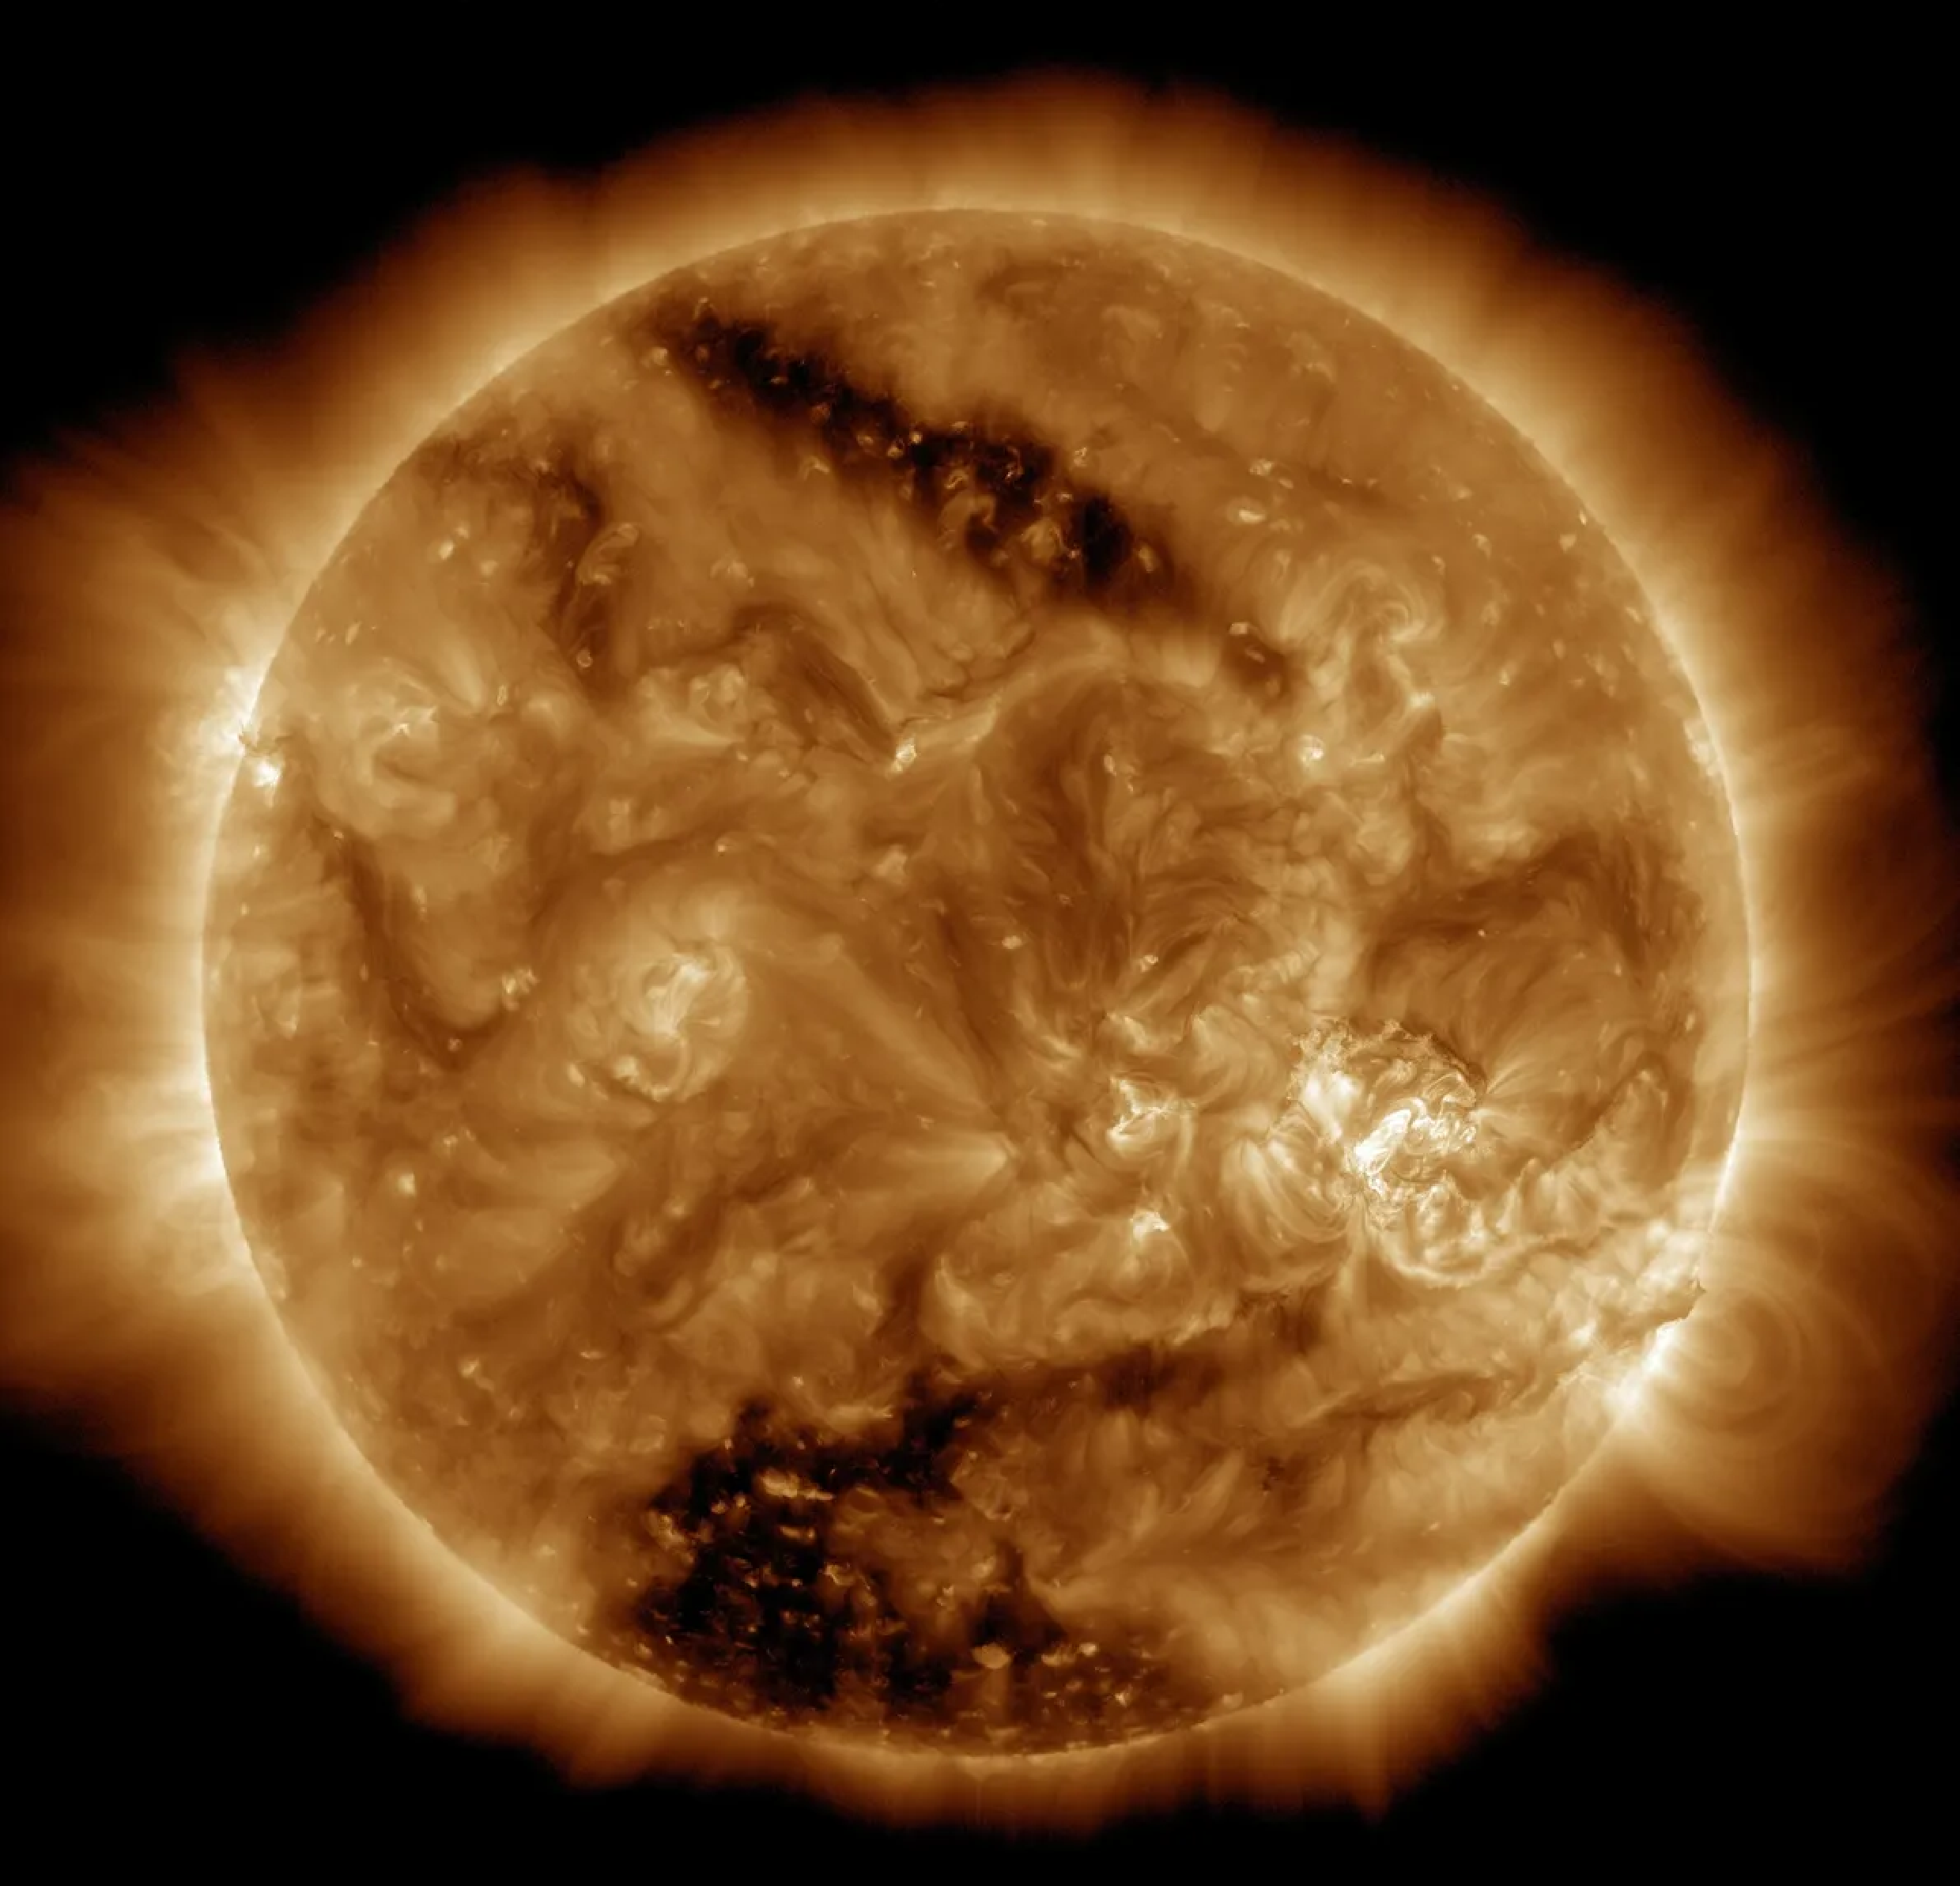
\includegraphics[width=0.6\textwidth,height=\textheight]{figures/grav/soleil.pdf}

}

\caption{Le soleil}

\end{figure}%

C'est à la fin du XVIe siècle qu'une avancée majeure est réalisée pour
expliquer le mouvement des astres : Johannes Kepler, sur base de mesures
méticuleuses réalisées par l'astronome danois Tycho Brahe, se rend
compte que les planètes ne décrivent pas des mouvements circulaires mais
elliptiques, dont un des foyers est occupé par le Soleil. Il s'agit de
sa première loi, parmi trois qui tentent de décrire le mouvement des
planètes autour du Soleil.

\begin{tcolorbox}[enhanced jigsaw, breakable, bottomrule=.15mm, colback=white, colframe=quarto-callout-note-color-frame, opacityback=0, arc=.35mm, left=2mm, toprule=.15mm, rightrule=.15mm, leftrule=.75mm]
\begin{minipage}[t]{5.5mm}
\textcolor{quarto-callout-note-color}{\faInfo}
\end{minipage}%
\begin{minipage}[t]{\textwidth - 5.5mm}

\vspace{-3mm}\textbf{Première loi: la loi des orbites.}\vspace{3mm}

La trajectoire de chaque planète est une ellipse dont un foyer est
occupé par le Soleil.

\end{minipage}%
\end{tcolorbox}

\begin{figure}[H]

{\centering 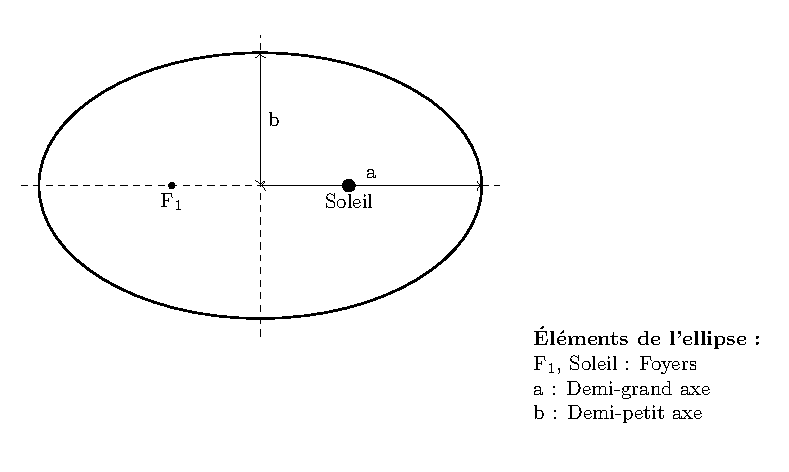
\includegraphics[width=0.8\textwidth,height=\textheight]{figures/grav/fig1.pdf}

}

\caption{Trajectoire elliptique}

\end{figure}%

\begin{tcolorbox}[enhanced jigsaw, breakable, bottomrule=.15mm, colback=white, colframe=quarto-callout-note-color-frame, opacityback=0, arc=.35mm, left=2mm, toprule=.15mm, rightrule=.15mm, leftrule=.75mm]
\begin{minipage}[t]{5.5mm}
\textcolor{quarto-callout-note-color}{\faInfo}
\end{minipage}%
\begin{minipage}[t]{\textwidth - 5.5mm}

\vspace{-3mm}\textbf{Deuxième loi: loi des aires.}\vspace{3mm}

Le segment qui joint le Soleil à une planète balaie des secteurs d'aires
égales en des durées égales, quelles que soient ces durées.

\end{minipage}%
\end{tcolorbox}

\begin{figure}[H]

{\centering 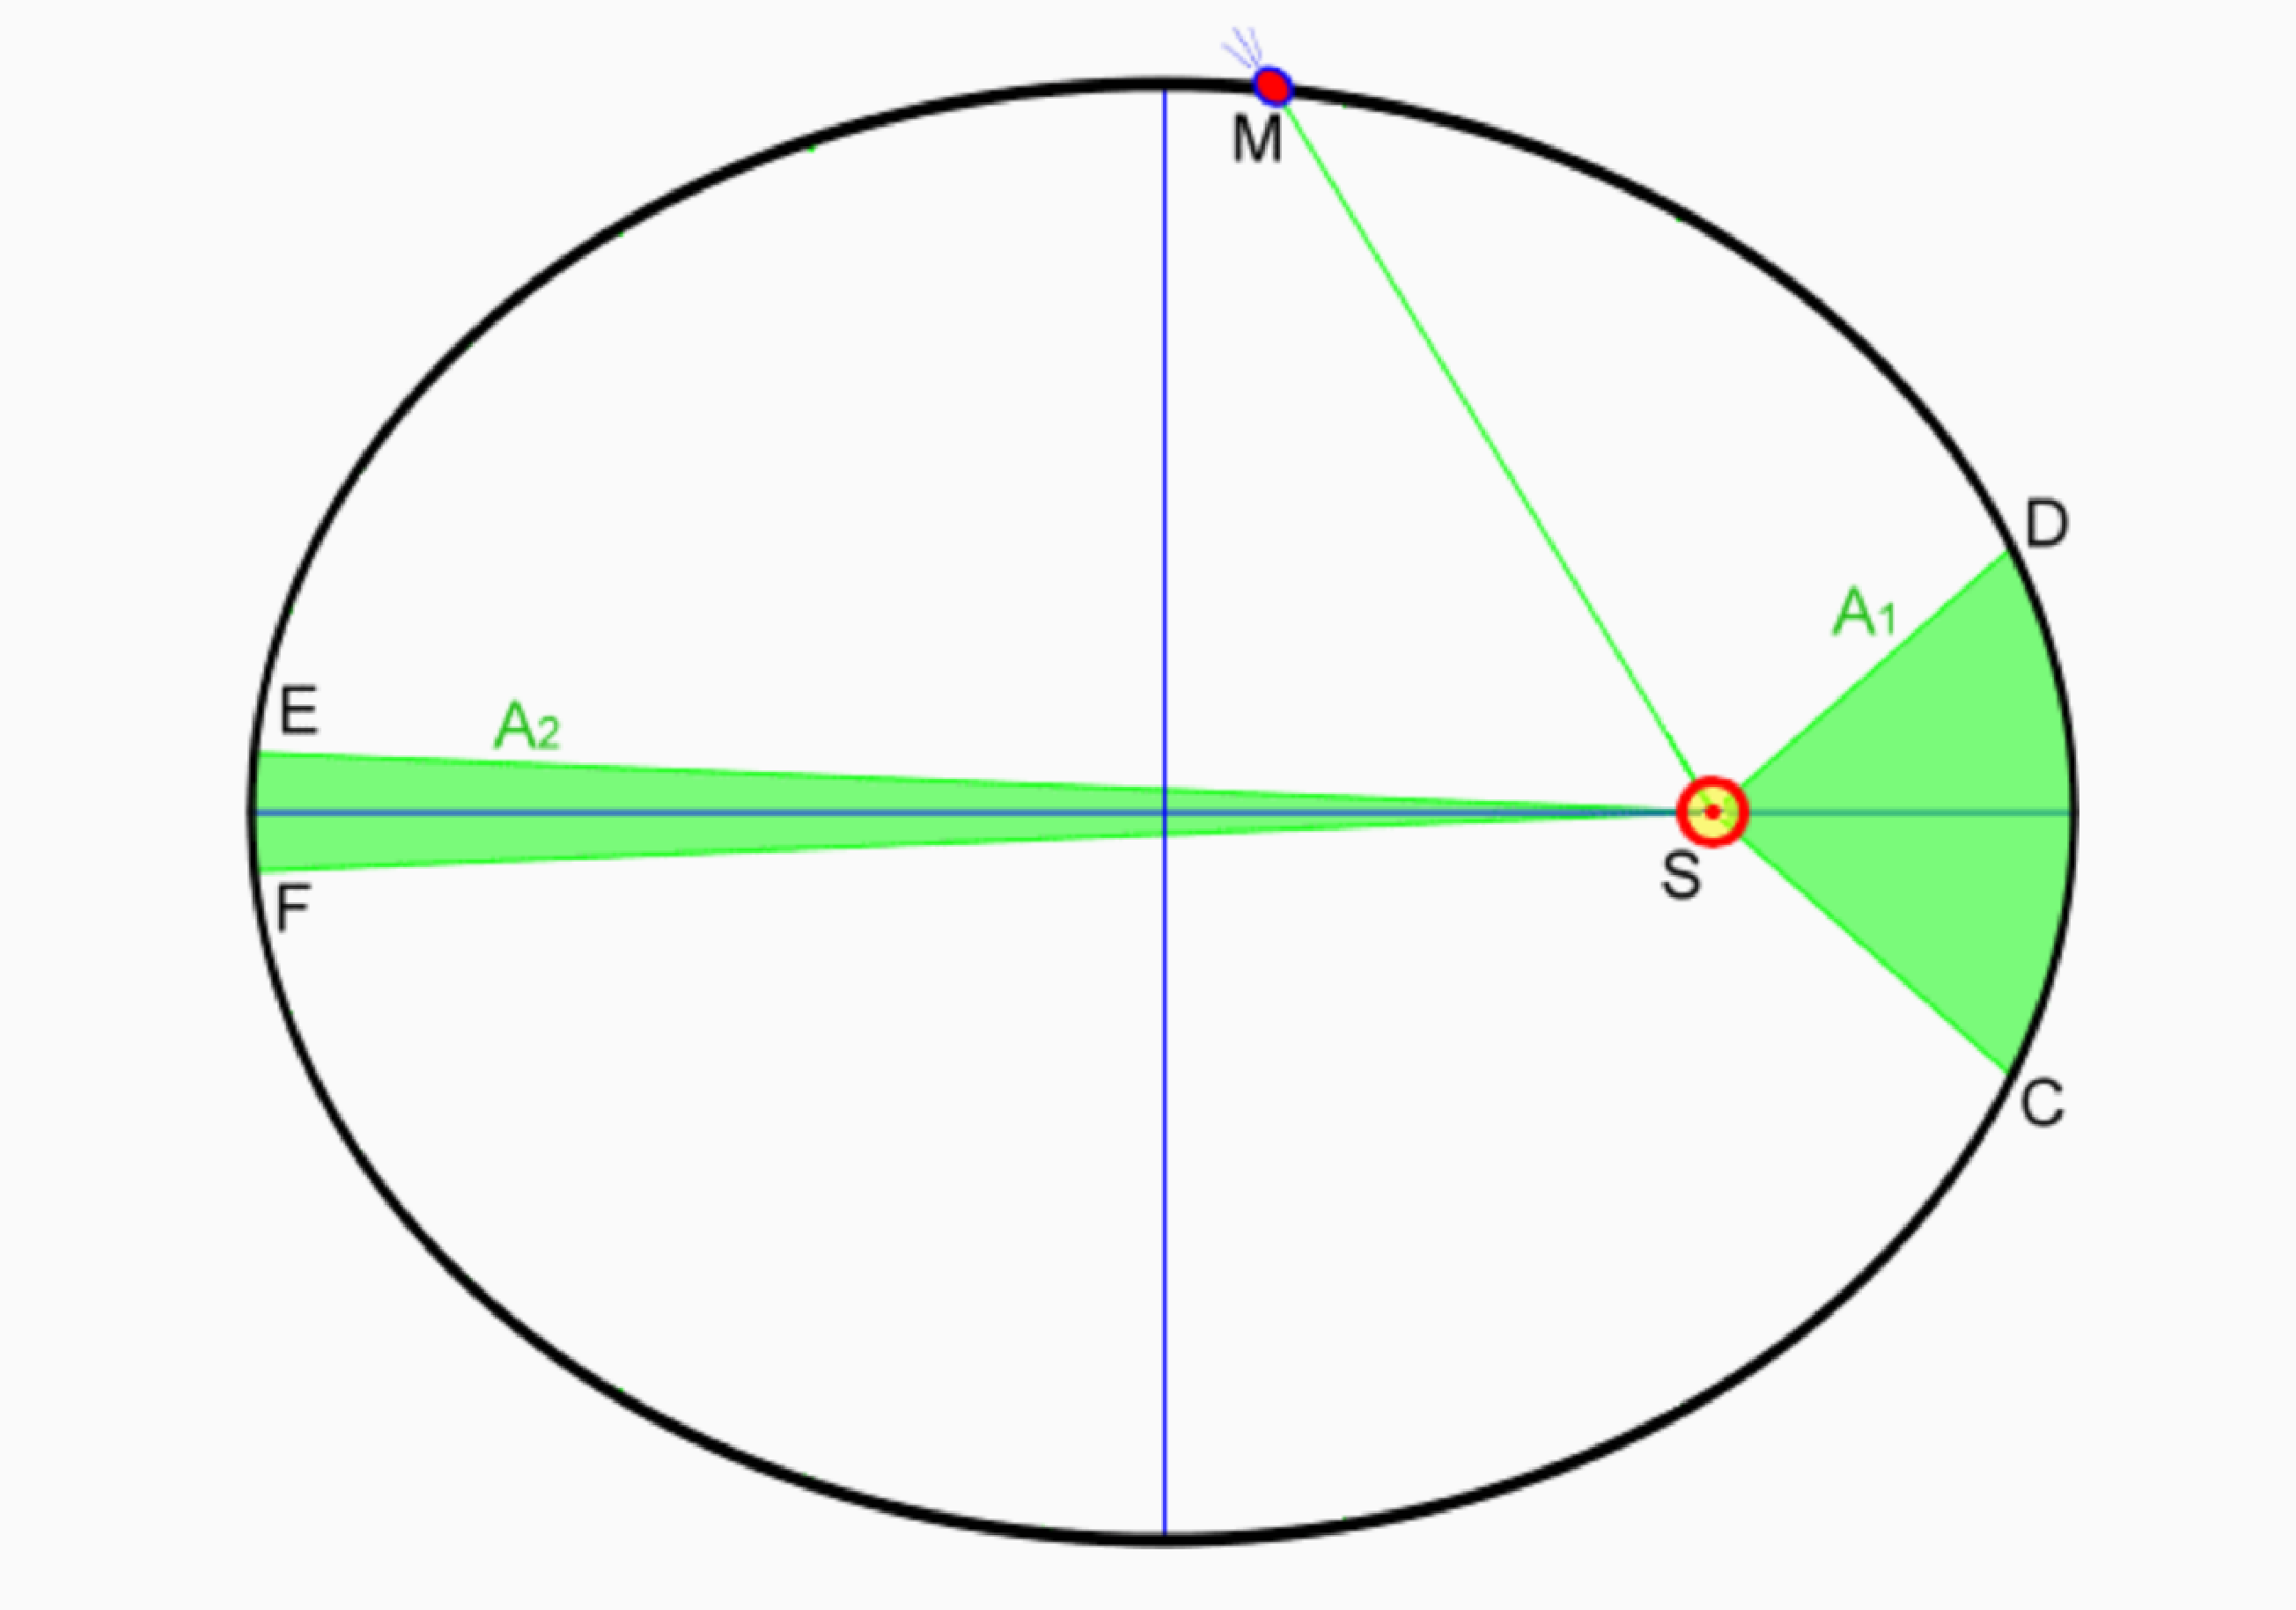
\includegraphics[width=0.8\textwidth,height=\textheight]{figures/grav/aires.pdf}

}

\caption{Loi des aires}

\end{figure}%

\begin{tcolorbox}[enhanced jigsaw, breakable, bottomrule=.15mm, colback=white, colframe=quarto-callout-note-color-frame, opacityback=0, arc=.35mm, left=2mm, toprule=.15mm, rightrule=.15mm, leftrule=.75mm]
\begin{minipage}[t]{5.5mm}
\textcolor{quarto-callout-note-color}{\faInfo}
\end{minipage}%
\begin{minipage}[t]{\textwidth - 5.5mm}

\vspace{-3mm}\textbf{Troisième loi: loi des périodes.}\vspace{3mm}

Le quotient du cube du demi-grand axe par le carré de la période de
révolution est le même pour toutes les planètes : \[
\frac{a^3_1}{T_1^2}=\frac{a^3_2}{T_2^2}=\ldots
\]

\end{minipage}%
\end{tcolorbox}

\begin{exercise}[]\protect\hypertarget{exr-kepler}{}\label{exr-kepler}

Complète le tableau suivant à l'aide de la 3e loi de Kepler.

\begin{longtable}[]{@{}
  >{\raggedright\arraybackslash}p{(\columnwidth - 6\tabcolsep) * \real{0.3100}}
  >{\raggedright\arraybackslash}p{(\columnwidth - 6\tabcolsep) * \real{0.2300}}
  >{\raggedright\arraybackslash}p{(\columnwidth - 6\tabcolsep) * \real{0.2300}}
  >{\raggedright\arraybackslash}p{(\columnwidth - 6\tabcolsep) * \real{0.2300}}@{}}
\toprule\noalign{}
\begin{minipage}[b]{\linewidth}\raggedright
Planète
\end{minipage} & \begin{minipage}[b]{\linewidth}\raggedright
\(a(10^9\text{m})\)
\end{minipage} & \begin{minipage}[b]{\linewidth}\raggedright
\(T(10^6\text{s})\)
\end{minipage} & \begin{minipage}[b]{\linewidth}\raggedright
\(a^3/T^3(10^{15}\text{m}^3/\text{s}^2)\)
\end{minipage} \\
\midrule\noalign{}
\endhead
\bottomrule\noalign{}
\endlastfoot
Mercure & 57,9 & & 3356 \\
Vénus & 108,1 & 19,41 & \\
Terre & 149,6 & & \\
Mars & & 59,36 & 3364 \\
Jupiter & 778,4 & 374,3 & \\
Saturne & 1424 & 928,4 & \\
\end{longtable}

\end{exercise}

\subsection{La loi de la gravitation
universelle}\label{la-loi-de-la-gravitation-universelle}

Kepler a décrit avec précision le mouvement des planètes, mais il ne l'a
pas expliqué. Il faut attendre le XVIIe siècle et Isaac Newton pour
comprendre pourquoi les planètes suivent ces trajectoires elliptiques.

\begin{figure}[H]

{\centering 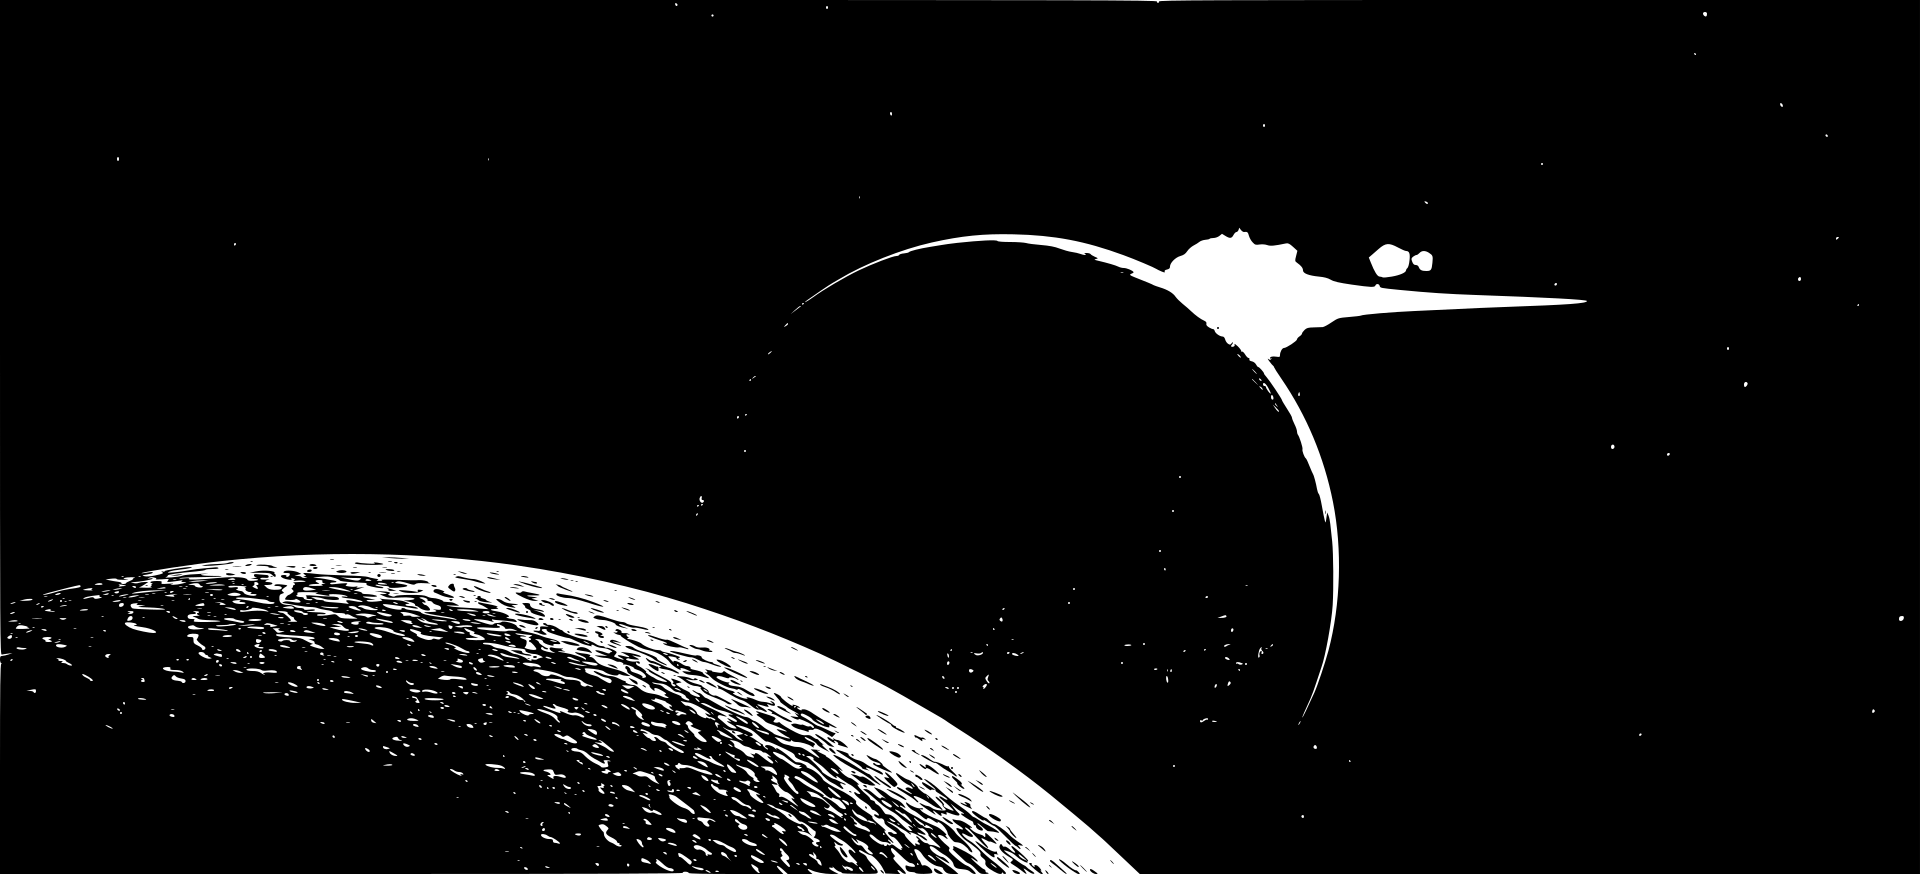
\includegraphics{figures/grav/terre-mune.pdf}

}

\caption{La terre vue de la Lune}

\end{figure}%

Newton propose que toutes les masses s'attirent mutuellement avec une
force qui dépend de certaines de leurs carctéristiques. Il va montrer
ainsi que l'interaction qui fait tomber un objet sur Terre est aussi
responsable du mouvement des planètes autour du Soleil. Cette idée
révolutionnaire unifie les phénomènes terrestres et célestes sous une
même loi.

Cette loi permet non seulement d'expliquer les trajectoires des planètes
décrites par Kepler, mais aussi d'autres phénomènes tels que la chute
des objets sur Terre, les marées ou encore le mouvement des satellites
artificiels.

Newton montre que les lois de Kepler sont une conséquence directe de la
gravitation universelle : en appliquant ses lois du mouvement et la
force gravitationnelle, il retrouve les trajectoires elliptiques des
planètes. C'est ainsi que la physique moderne voit le jour : un même
principe explique à la fois le mouvement des corps célestes et celui des
objets terrestres.

\begin{figure}[H]

{\centering 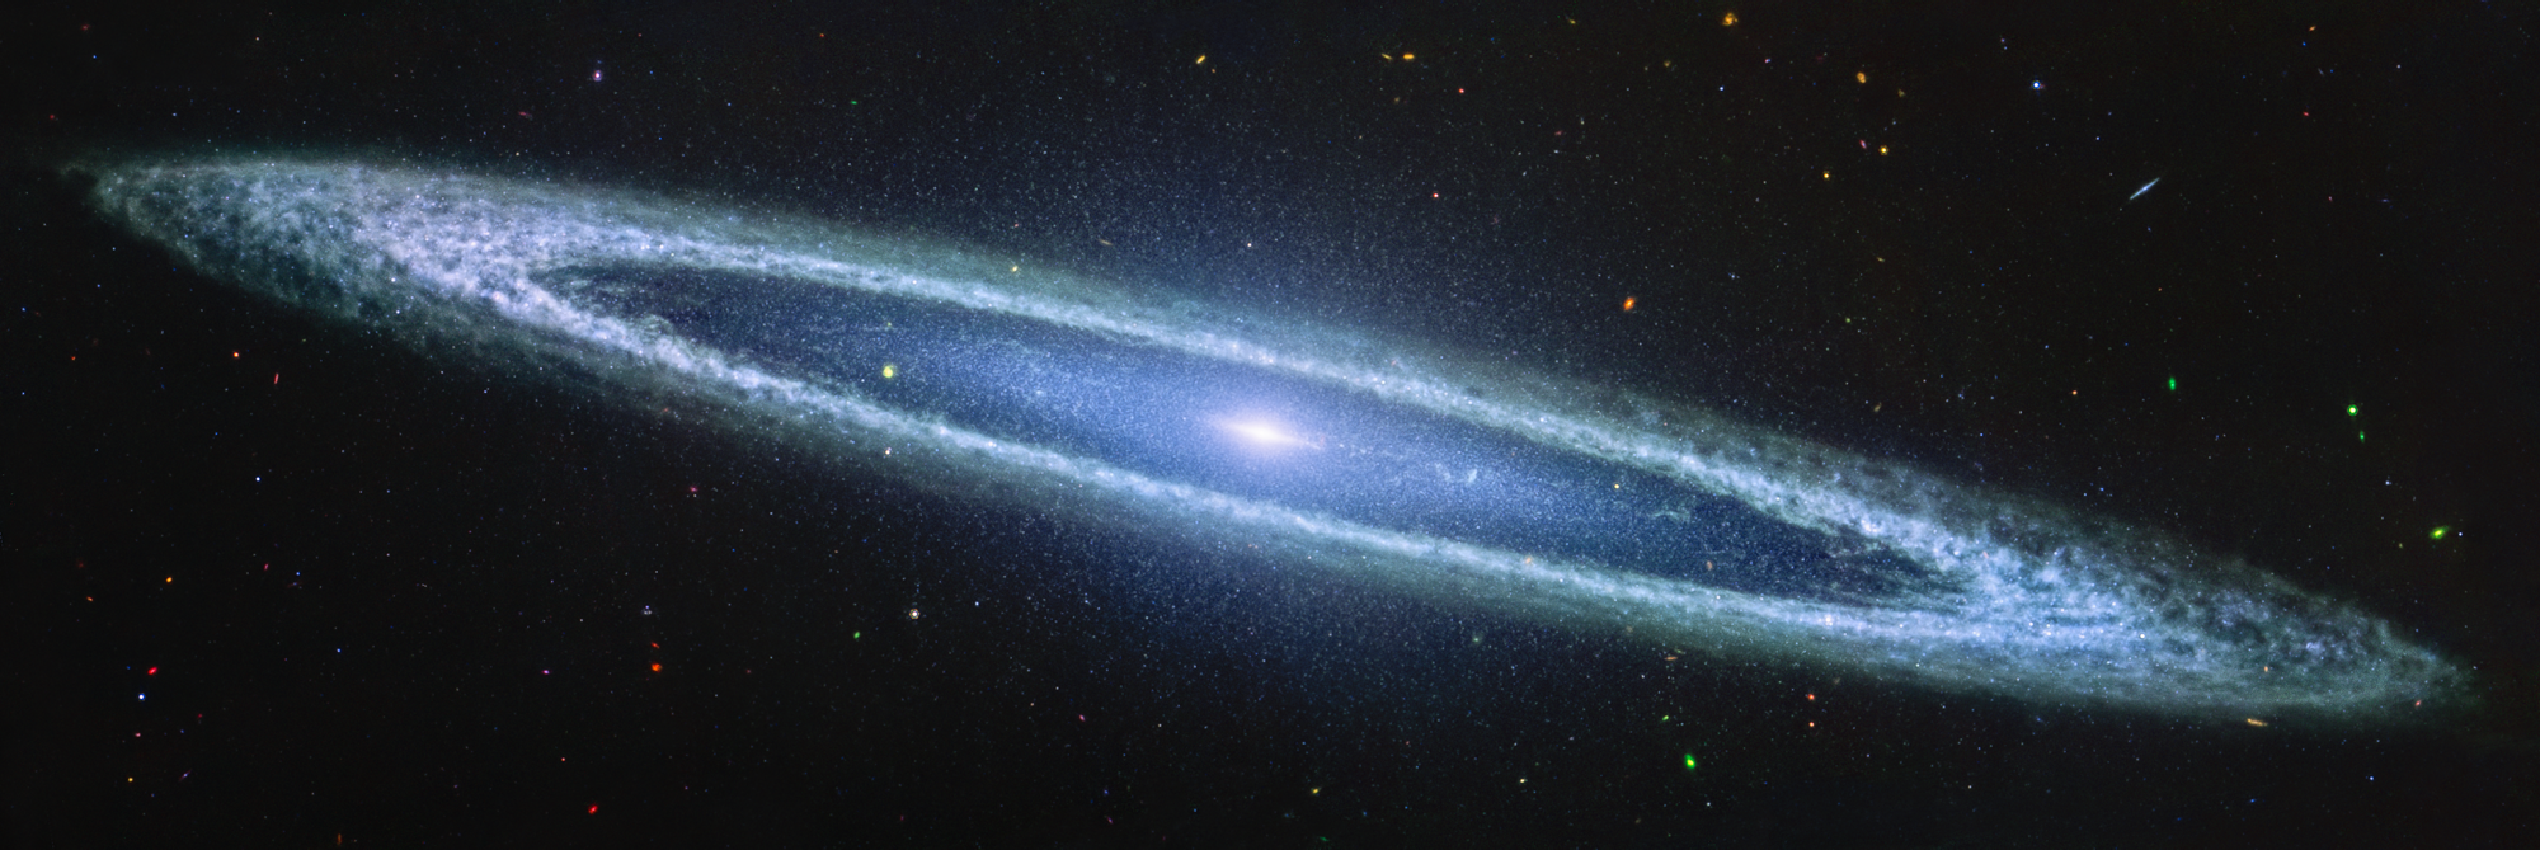
\includegraphics{figures/grav/galaxie-sombrero.pdf}

}

\caption{La galaxie du sombrero}

\end{figure}%

\section{La loi de la gravitation
universelle}\label{la-loi-de-la-gravitation-universelle-1}

\subsection{La démarche de Newton}\label{la-duxe9marche-de-newton}

Nous allons énoncer la loi de la gravitation universelle en suivant la
démarche de Newton.

La première idée de Newton est d'interpréter le mouvement de la Lune
autour de la Terre comme une chute libre. Voici une animation qui
illustre cette interprétation :

\begin{figure}[H]

{\centering 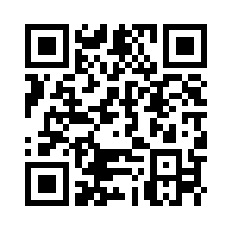
\includegraphics[width=0.2\textwidth,height=\textheight]{figures/grav/sat.pdf}

}

\caption{QR-code de l'application}

\end{figure}%

Tout objet proche de la surface de la Terre est soumis à une force
gravitationnelle. Par exemple, une pomme que vous tenez dans la main
subit une accélération dirigée vers le centre de la Terre, d'intensité
\(g = 9,81\text{ m/s}^2\). Si vous lâchez cette pomme, elle tombe. Si
vous la lancez horizontalement, elle suit une trajectoire parabolique.

En s'appuyant sur cette idée, Newton a imaginé un tir horizontal où la
vitesse initiale est si grande que l'objet ne retombe jamais au sol. La
Lune, selon cette vision, est en perpétuelle chute libre autour de la
Terre, mais sa vitesse lui permet de « manquer » la Terre en permanence.

Les observations montrent que la trajectoire de la Lune est
approximativement circulaire. Nous allons donc supposer dans la suite
qu'elle décrit un mouvement circulaire uniforme (MCU) autour de la
Terre, avec une vitesse d'intensité constante. Ce modèle implique que la
Lune possède une accélération centripète \(a_L\), que nous allons
comparer à l'accélération d'un objet en chute libre sur Terre.

\begin{figure}[H]

{\centering 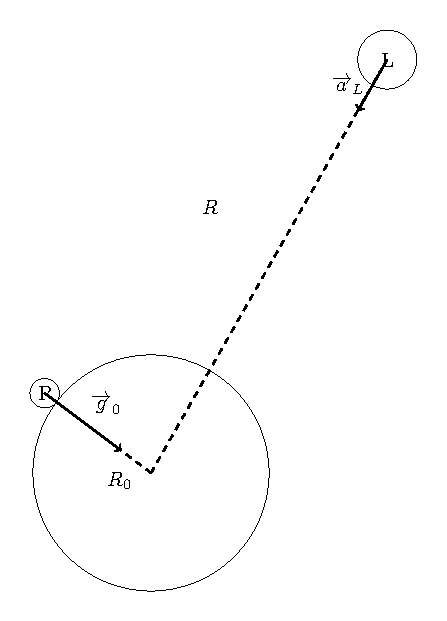
\includegraphics[width=0.5\textwidth,height=\textheight]{figures/grav/fig3.pdf}

}

\caption{La Pomme de Newton et la Lune}

\end{figure}%

Pour rappel :

\begin{enumerate}
\def\labelenumi{\arabic{enumi}.}
\tightlist
\item
  \(a_L = \omega^2 R = \dfrac{4\pi^2 R}{T^2}\)
\item
  Le rayon Terre-Lune est \(R = 385 000\) km
\item
  Le rayon de la Terre est \(R_0 = 6370\) km
\end{enumerate}

\begin{exercise}[]\protect\hypertarget{exr-lune}{}\label{exr-lune}

~

\begin{enumerate}
\def\labelenumi{\arabic{enumi}.}
\tightlist
\item
  Calculer \(\dfrac{g}{a_L}\).
\item
  Calculer \(\dfrac{R}{R_0}\).
\item
  Déduire que \(\dfrac{g}{a_L} \simeq \left(\dfrac{R}{R_0}\right)^2\).
\end{enumerate}

\end{exercise}

Newton en déduit que la force exercée par la Terre sur la pomme,
\(\overrightarrow{F}_{\text{T/P}}\), est de même nature que celle
exercée sur la Lune, \(\overrightarrow{F}_{\text{T/L}}\). Les résultats
de l'exercice précédent montrent que cette force est proportionnelle à
\(\dfrac{1}{R^2}\).

\begin{tcolorbox}[enhanced jigsaw, breakable, bottomrule=.15mm, colback=white, colframe=quarto-callout-important-color-frame, opacityback=0, arc=.35mm, left=2mm, toprule=.15mm, rightrule=.15mm, leftrule=.75mm]
\begin{minipage}[t]{5.5mm}
\textcolor{quarto-callout-important-color}{\faExclamation}
\end{minipage}%
\begin{minipage}[t]{\textwidth - 5.5mm}

\vspace{-3mm}\textbf{Dépendance de la distance}\vspace{3mm}

Autrement dit, l'intensité de la force d'attraction terrestre diminue
avec le carré de la distance au centre de la Terre.

\end{minipage}%
\end{tcolorbox}

D'après la deuxième loi de Newton, la force gravitationnelle
\(\overrightarrow{F}_{\text{T/L}}\) est reliée à l'accélération de la
Lune par :

\[
\overrightarrow{F}_{\text{T/L}} = m_L \overrightarrow{a}_L.
\]

On en déduit que cette force dépend de la masse de la Lune, \(m_L\).

Un autre paramètre intervient : la masse de la Terre, \(m_T\). En effet,
selon la loi des actions réciproques, la Lune exerce également une force
sur la Terre, \(\overrightarrow{F}_{\text{L/T}}\). Ces deux forces sont
opposées mais de même intensité :

\[
\overrightarrow{F}_{\text{T/L}} = -\overrightarrow{F}_{\text{L/T}}.
\]

D'après la deuxième loi de Newton, \(\overrightarrow{F}_{\text{T/L}}\)
dépend donc aussi de la masse de la Terre.

\begin{figure}[H]

{\centering 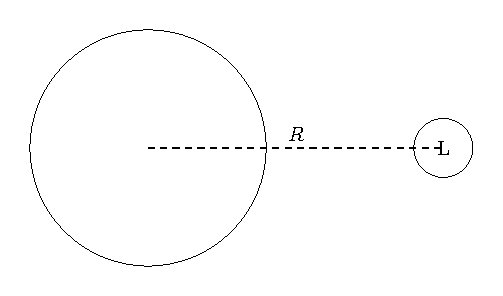
\includegraphics[width=0.6\textwidth,height=\textheight]{figures/grav/fig4.pdf}

}

\caption{L'attraction de la Lune par la Terre}

\end{figure}%

\subsection{L'énoncé de la loi de la gravitation
universelle}\label{luxe9noncuxe9-de-la-loi-de-la-gravitation-universelle}

En résumé, la force \(\overrightarrow{F}_{\text{T/L}}\) est :

\begin{enumerate}
\def\labelenumi{\arabic{enumi}.}
\tightlist
\item
  proportionnelle aux masses \(m_L\) et \(m_T\),
\item
  inversement proportionnelle au carré de la distance \(R\) entre les
  deux corps.
\end{enumerate}

Le génie de Newton a été d'étendre ce raisonnement à tous les astres du
système solaire, puis à tous les corps matériels. Il en a déduit une loi
fondamentale de la nature.

\begin{tcolorbox}[enhanced jigsaw, breakable, bottomrule=.15mm, colback=white, colframe=quarto-callout-note-color-frame, opacityback=0, arc=.35mm, left=2mm, toprule=.15mm, rightrule=.15mm, leftrule=.75mm]
\begin{minipage}[t]{5.5mm}
\textcolor{quarto-callout-note-color}{\faInfo}
\end{minipage}%
\begin{minipage}[t]{\textwidth - 5.5mm}

\vspace{-3mm}\textbf{Loi de la gravitation universelle}\vspace{3mm}

Deux corps ponctuels s'attirent avec une force dirigée selon la droite
qui les joint. L'intensité de cette force est proportionnelle au produit
de leurs masses et inversement proportionnelle au carré de la distance
qui les sépare :

\[
F_{m_1/m_2}=F_{m_2/m_1} = k_g \dfrac{m_1 m_2}{R^2}.
\]

\end{minipage}%
\end{tcolorbox}

\begin{center}
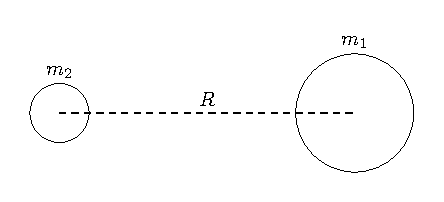
\includegraphics[width=0.6\textwidth,height=\textheight]{figures/grav/fig7.pdf}
\end{center}

La constante \(k_g\) est universelle. Elle a été estimée par Newton et
mesurée avec précision par Cavendish en 1798 :

\[
k_g = 6,67 \times 10^{-11} \dfrac{\text{N} \cdot \text{m}^2}{\text{kg}^2}.
\]

Cette valeur montre que la force gravitationnelle est généralement
faible. Elle diminue rapidement lorsque la distance entre les objets
augmente. Pour mieux comprendre cette relation, représentons
graphiquement la variation de la force gravitationnelle entre deux
objets en fonction de leur distance.\\
On choisi deux masses \(m_1=m_2=m\) de sorte à ce que \(k_gm^2=1\). Ceci
permet d'écrire que \(F_{m_1/m_2}=\dfrac{1}{R^2}\). Voici une
représentation graphique de \(F_{m_1/m_2}\) en fonction de la distance
entre les objets.

\begin{figure}[H]

{\centering 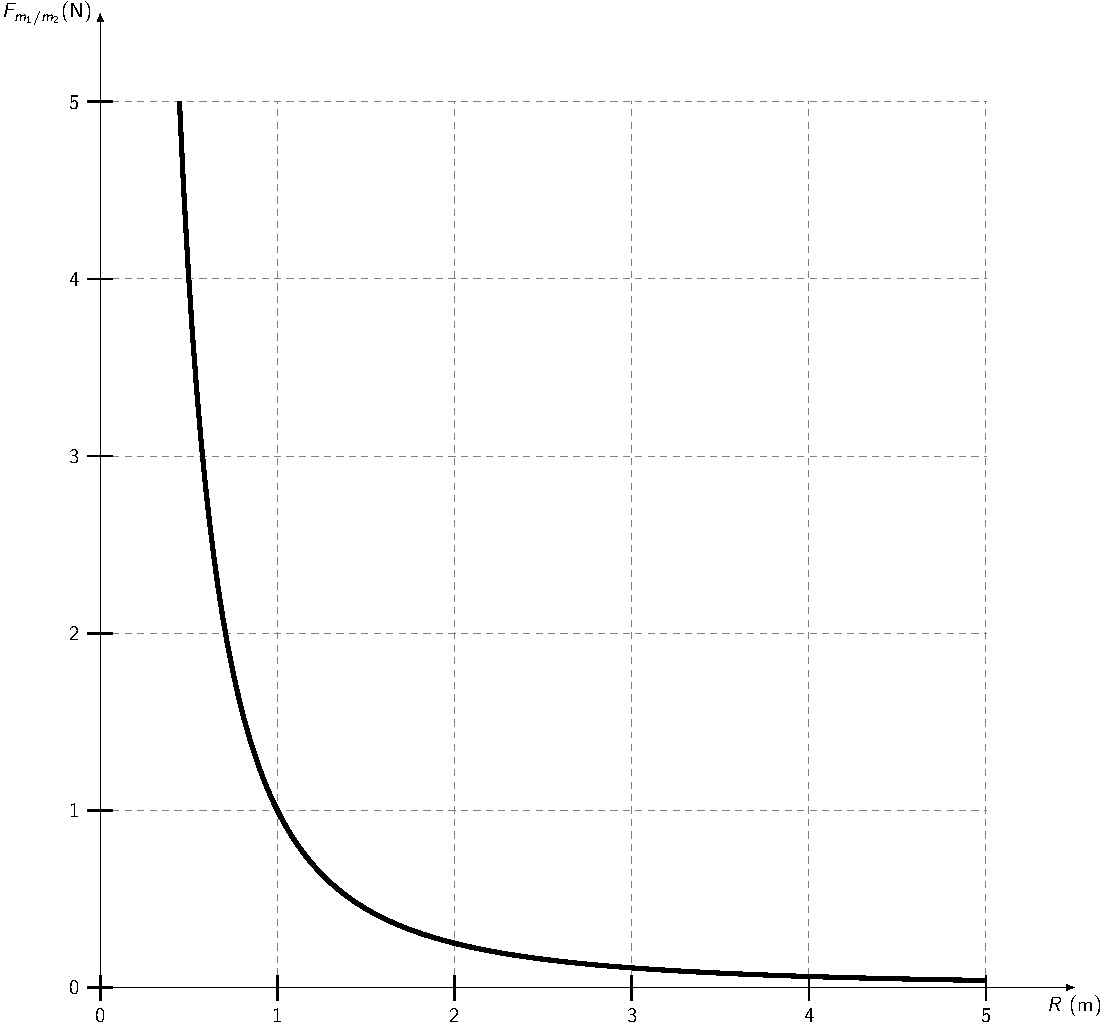
\includegraphics[width=0.6\textwidth,height=\textheight]{figures/grav/fig02.pdf}

}

\caption{Intensité de la force en fonction de la distance}

\end{figure}%

\begin{exercise}[]\protect\hypertarget{exr-refl}{}\label{exr-refl}

~

\begin{enumerate}
\def\labelenumi{\arabic{enumi}.}
\tightlist
\item
  Si la distance entre deux objets double, comment est modifiée la force
  gravitationnelle entre eux ?
\item
  Un astronaute lâche un objet en chute libre sur une planète inconnue.
  Son accélération augmente-t-elle au cours de la chute ?
\item
  Le poids d'un kilogramme de plumes est-il le même sur la Terre et sur
  la Lune ? Justifier.
\end{enumerate}

\end{exercise}

\begin{exercise}[]\protect\hypertarget{exr-appl}{}\label{exr-appl}

Calcule la force d'attraction que tu exerces sur ton voisin le plus
proche. Explique ensuite pourquoi tu n'est pas collé à ton voisin.

\end{exercise}

\subsection{Applications}\label{applications}

Pour les exercices qui suivent, les constantes suivantes seront
utilisées.

\begin{longtable}[]{@{}
  >{\raggedright\arraybackslash}p{(\columnwidth - 2\tabcolsep) * \real{0.5789}}
  >{\raggedright\arraybackslash}p{(\columnwidth - 2\tabcolsep) * \real{0.4211}}@{}}
\toprule\noalign{}
\begin{minipage}[b]{\linewidth}\raggedright
Constante
\end{minipage} & \begin{minipage}[b]{\linewidth}\raggedright
Valeur
\end{minipage} \\
\midrule\noalign{}
\endhead
\bottomrule\noalign{}
\endlastfoot
Constante gravitationnelle \(k_g\) &
\(6,67 \times 10^{-11} \frac{\text{N} \cdot \text{m}^2}{\text{kg}^2}\) \\
Accélération terrestre \(g\) & \(9,81 \text{ m/s}^2\) \\
Masse de la Terre \(m_T\) & \(5,97 \times 10^{24} \text{ kg}\) \\
Masse du Soleil \(m_S\) & \(1,99 \times 10^{30} \text{ kg}\) \\
Rayon de la Terre \(R_T\) & \(6,37 \times 10^6\) m \\
Distance Terre-Soleil \(R_{TS}\) & \(1,5\times 10^{11}\) m \\
\end{longtable}

\subsection{Mouvement des astres dans le système
solaire}\label{mouvement-des-astres-dans-le-systuxe8me-solaire}

La première loi de Kepler dit que la trajectoire des planètes autour du
soleil est elliptique. Voici une représentation de quelques unes de ces
trajectoires:

\begin{figure}[H]

{\centering 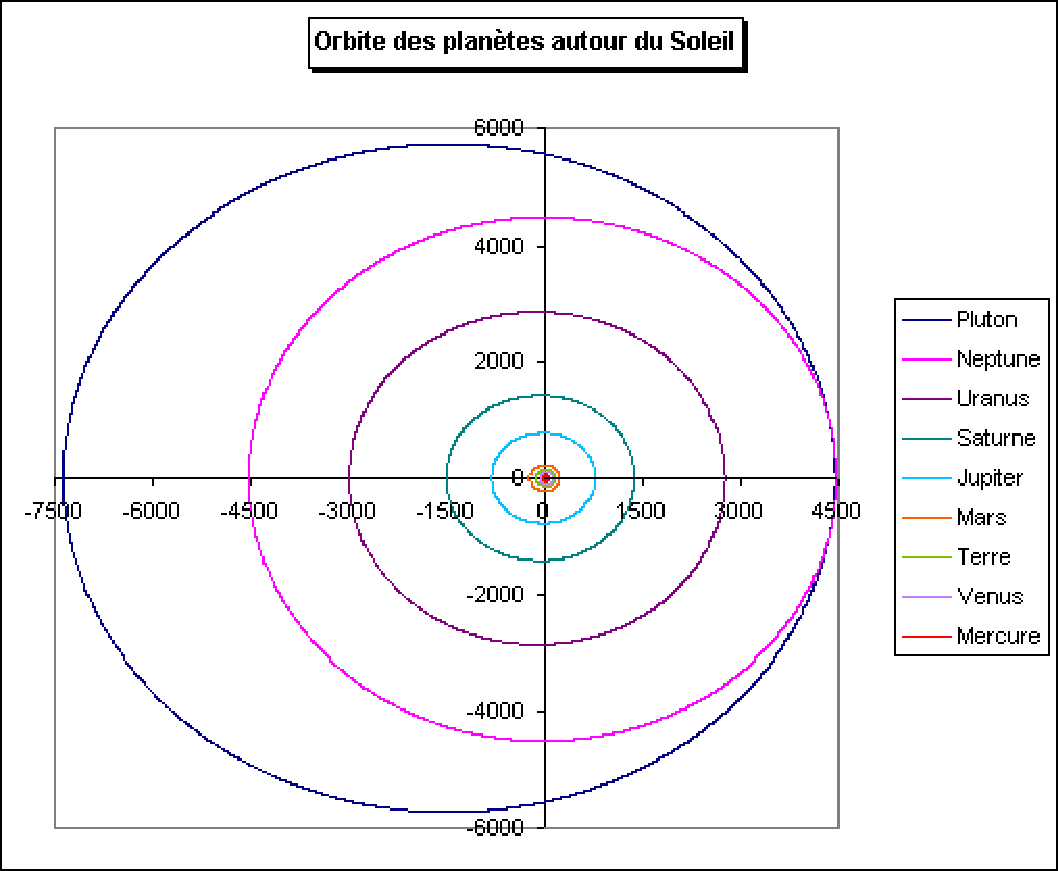
\includegraphics[width=0.2\textwidth,height=\textheight]{figures/grav/orbites.pdf}

}

\caption{Orbites du système solaire (échelle: \(10^9\)m)}

\end{figure}%

Tu peux constater que les trajectoires ont l'air d'être des cercles.
Nous supposerons donc, afin de faciliter les calculs, que les
trajectoires des astres dans le système solaire sont circulaires. Ceci
nous permettra de faire appel à la théorie des MCU pour résoudre les
exercices.

Voyons un exemple d'application pour trouver la vitesse ou la période de
révolution d'un astre.

\begin{example}[]\protect\hypertarget{exm-netpune}{}\label{exm-netpune}

Dans cet exemple, nous allons estimer la vitesse orbitale de Neptune, en
sachant que le rayon de l'orbite de Neptune autour du soleil est
\(4 498 400 000 \text{km}=4,4984\cdot 10^{12}\) m.

Explicitons ce que dit l'énoncé de l'exemple:

\begin{enumerate}
\def\labelenumi{\arabic{enumi}.}
\tightlist
\item
  \(F_{S/N}=k_g\dfrac{m_Sm_N}{R_N^2}\);
\item
  \(R_N=4,4984\cdot 10^{12}\) m.
\end{enumerate}

D'après la deuxième loi de Newton, on a que \(F_{S/N}=m_Na_N\) , où
\(a_N=\dfrac{v^2}{R_N}\) est l'accélération centripète.

On a donc \(v^2=k_g\dfrac{m_S}{R_N}\). Comme
\(R_N=30 R_T=30\cdot 6,37\cdot 10^6\text{m}\), on a que

\[
v^2=6,67\cdot 10^{-11}\dfrac{1,99\cdot 10^{30}}{4,4984\cdot 10^{12}}=29506713,5 \text{m}^2/\text{s}^2.
\]

Donc \(v\simeq 5432\text{m/s}=19555,2\text{km/h}\).

\end{example}

\begin{exercise}[]\protect\hypertarget{exr-vitesse-orbitale}{}\label{exr-vitesse-orbitale}

Un satellite artificiel tourne autour de la Terre à une altitude de 500
km.

\begin{enumerate}
\def\labelenumi{\arabic{enumi}.}
\tightlist
\item
  Exprime le rayon de son orbite en fonction du rayon terrestre.
\item
  Calcule sa vitesse orbitale.
\item
  Donne la période de révolution du satellite.
\end{enumerate}

\end{exercise}

\begin{exercise}[]\protect\hypertarget{exr-iss}{}\label{exr-iss}

La station spatiale internationale (ISS) est en orbite circulaire autour
de la Terre à une altitude de 400km. Calcule la vitesse de l'ISS.

\end{exercise}

\begin{figure}[H]

{\centering 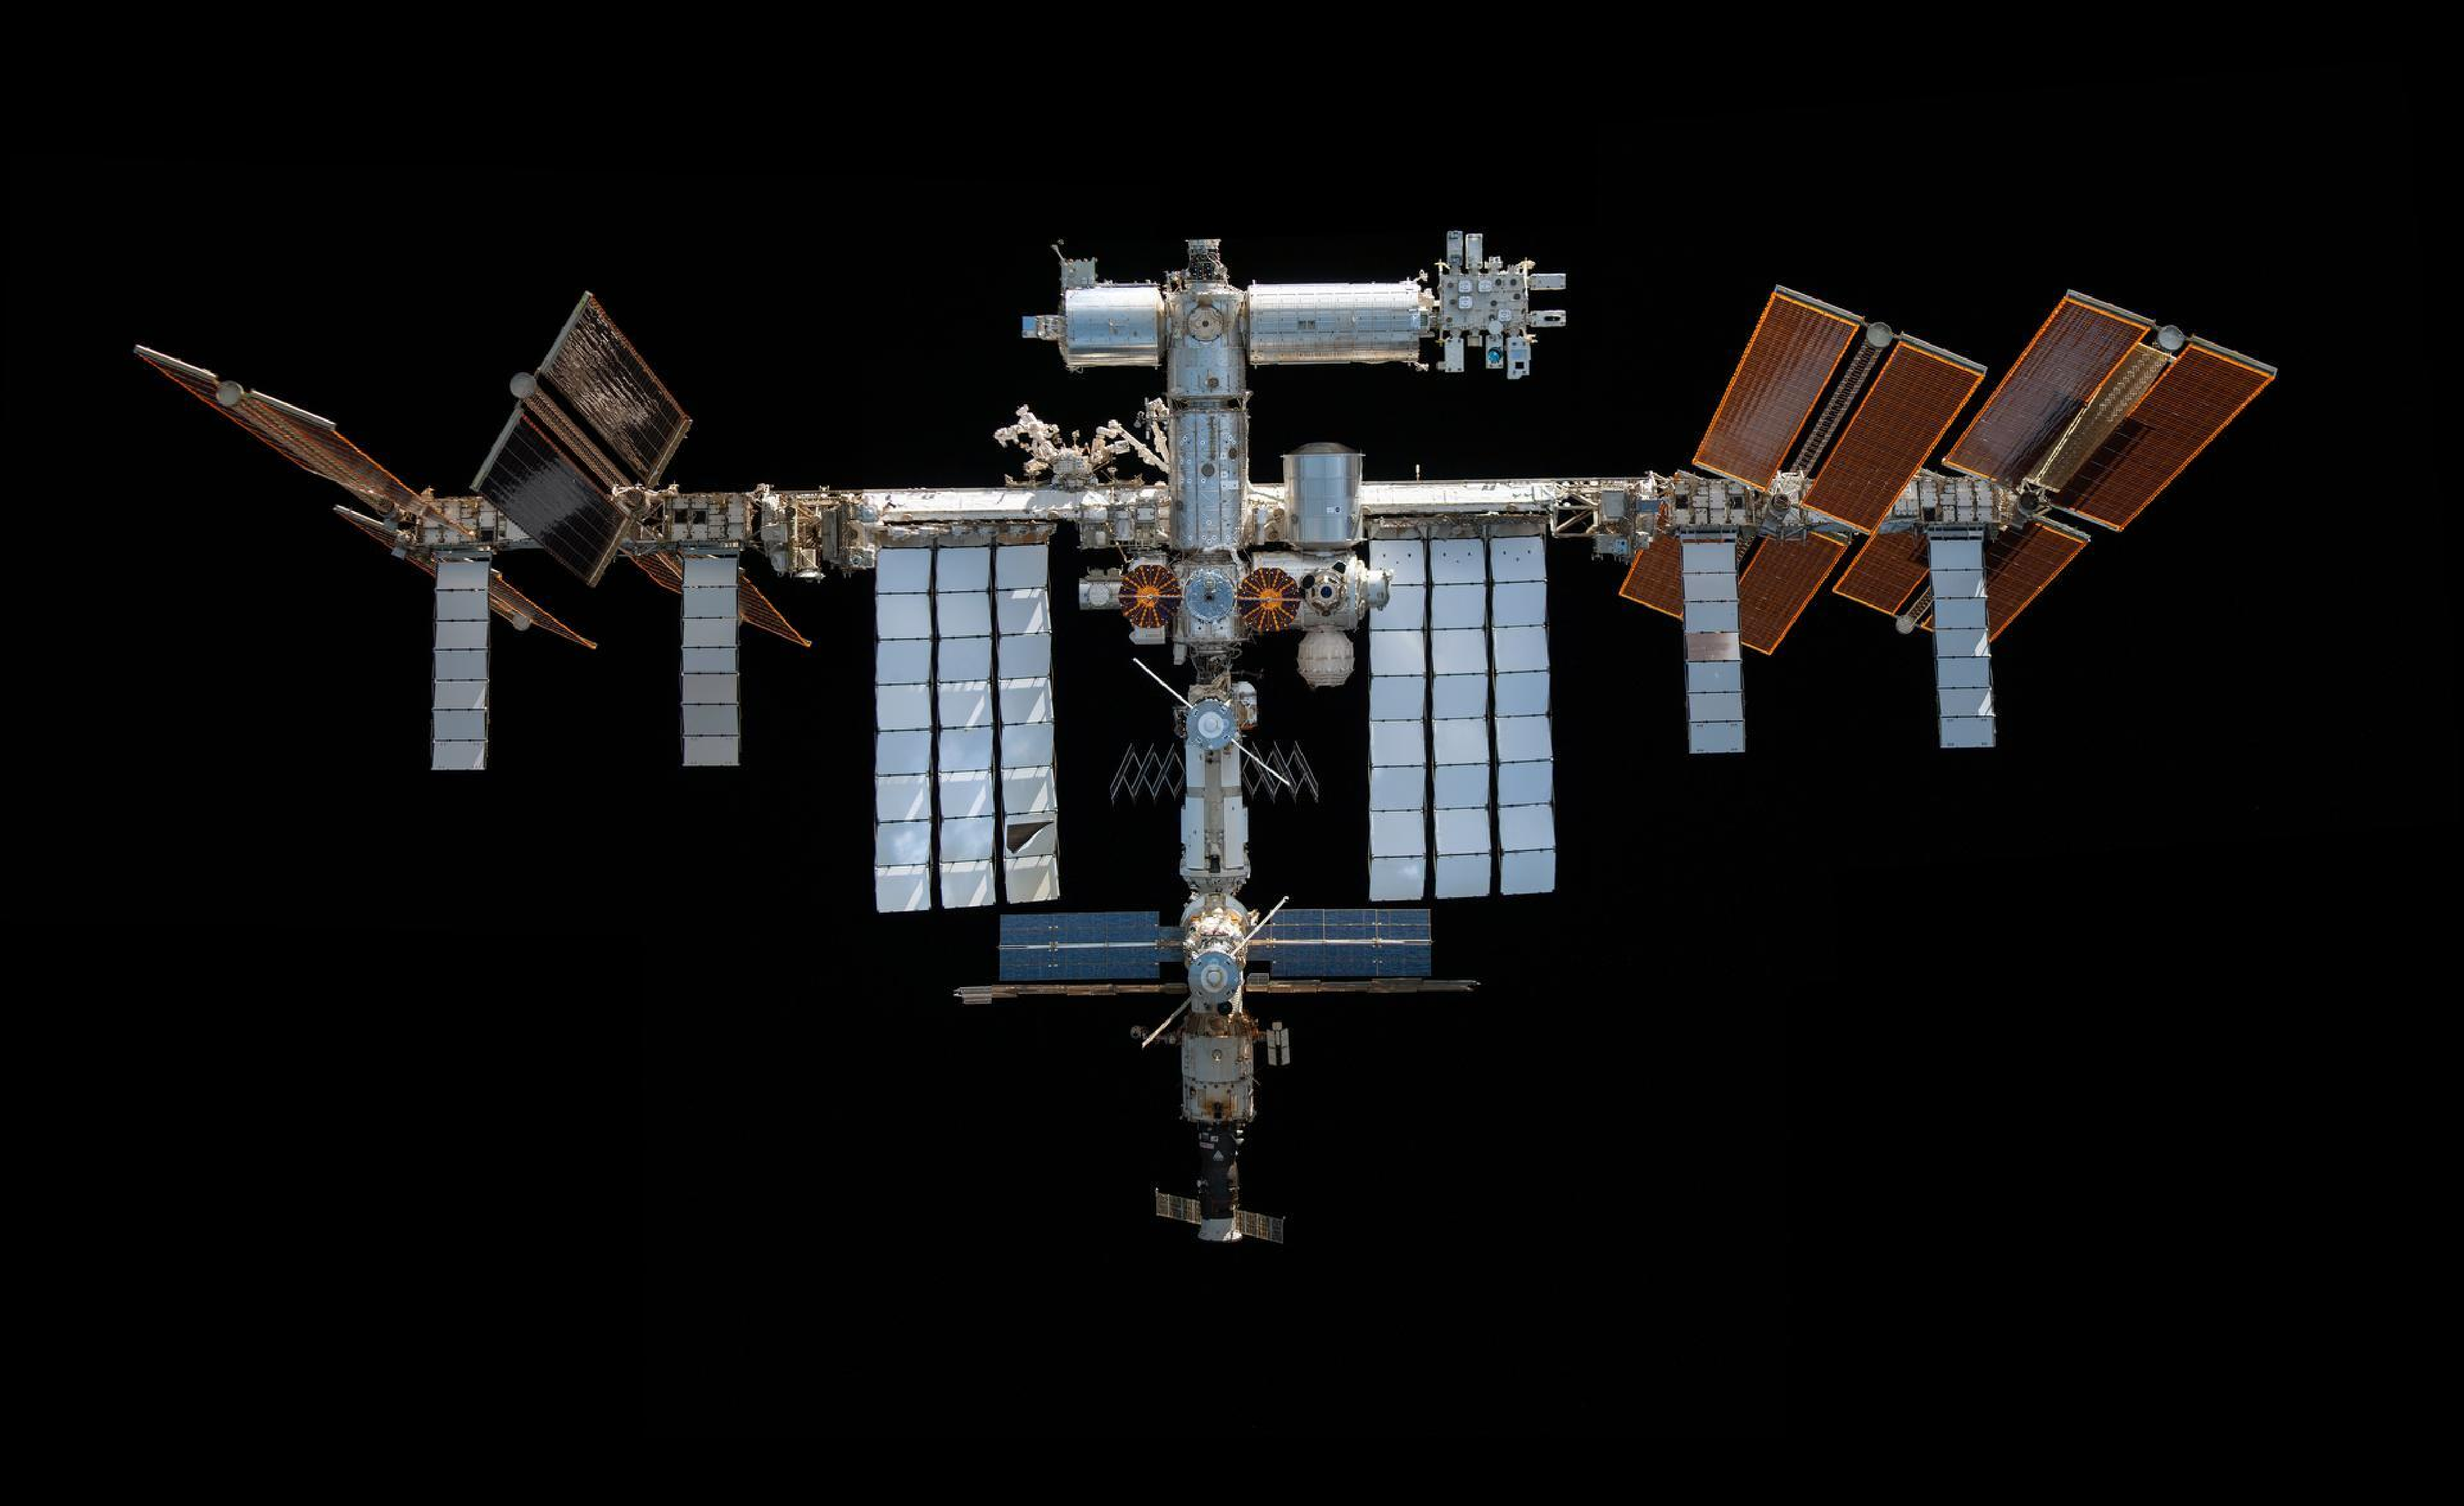
\includegraphics[width=0.4\textwidth,height=\textheight]{figures/grav/iss.pdf}

}

\caption{L'ISS}

\end{figure}%

\section{Détermination de la masse des corps
célestes}\label{duxe9termination-de-la-masse-des-corps-cuxe9lestes}

La loi de la gravitation est une des seules manières dont nous pouvons
mesurer la masse des astres.

Prenons l'exemple de la Terre. Comment peut-on déterminer sa masse sans
avoir à la ``peser'' directement ?

L'idée repose sur la relation entre la force gravitationnelle et
l'accélération gravitationnelle \(g\).

Nous savons que tout objet de masse \(m\) situé près de la surface
terrestre subit une accélération \(g = 9,81\) m/s². Cette accélération
est due à la force gravitationnelle exercée par la Terre.

En appliquant la deuxième loi de Newton :

\[
m g =  k_g\frac{m m_T}{R_T^2}
\]

On peut simplifier :

\[
g = k_g\frac{ m_T}{R_T^2}
\]

D'où :

\[
m_T = \frac{g R_T^2}{k_g}\simeq 5,97\cdot 10^{24}\text{kg}.
\]

Ce raisonnement nous permet de déterminer la masse de n'importe quel
astre en connaissant son rayon et son influence sur un objet en orbite
autour de lui ou à sa surface.

\begin{exercise}[]\protect\hypertarget{exr-masse-terre}{}\label{exr-masse-terre}

En utilisant \(g_M = 3,71\) m/s² et \(R_M = 3,39 \times 10^6\) m,
calcule la masse de Mars.

\end{exercise}

\begin{exercise}[]\protect\hypertarget{exr-masse-mars}{}\label{exr-masse-mars}

Le but de cet exercice est de calculer la masse du Soleil, sur base du
mouvement de la Terre.

\begin{enumerate}
\def\labelenumi{\arabic{enumi}.}
\tightlist
\item
  Calcule la vitesse de la terre autour du soleil.
\item
  Déduis-en la masse du Soleil.
\end{enumerate}

\end{exercise}

\section{La gravité autour de la
Terre}\label{la-gravituxe9-autour-de-la-terre}

L'accélération gravitationnelle varie avec l'altitude.

\begin{exercise}[]\protect\hypertarget{exr-alt}{}\label{exr-alt}

Considérons une bille de plomb de 1kg. Calcule la force de gravitation
exercée par la Terre sur cette masse si:

\begin{enumerate}
\def\labelenumi{\arabic{enumi}.}
\tightlist
\item
  elle est à 10m au dessus de la surface de la Terre.
\item
  elle est à 10km au dessus de la surface de la Terre.
\item
  elle est dans la Station Spaciale Internationale (400km d'altitude).
\end{enumerate}

\end{exercise}

Les calculs réalisés dans l'exercice précédent peuvent se généraliser
pour un objet de masse \(m\) à une altitude \(h\):

\begin{figure}[H]

{\centering 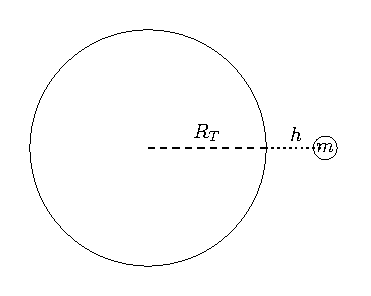
\includegraphics[width=0.8\textwidth,height=\textheight]{figures/grav/fig5.pdf}

}

\caption{Accélération gravitationnelle en fonction de l'altitude}

\end{figure}%

Pour cet objet, s'il est à la surface de la Terre, nous avons
\(g = \frac{k_g m_T}{R_T^2}=9,81 \text{m/s}^2\). Mais si l'objet est à
une altitude \(h\), la distance qui le sépare du centre de la Terre
devient \(R_T + h\). En notant \(g_h\) son accélération centripète, on
obtient:

\[
mg_h=k_g\dfrac{m_Tm}{(R_T+h)^2}.
\]

La nouvelle accélération gravitationnelle est donc :

\[
g_h = \frac{k_g m_T}{(R_T + h)^2}
\]

Ainsi on constate à nouveau que plus on s'éloigne de la Terre, plus
l'intensité de la force de gravité terrestre diminue.

\begin{exercise}[]\protect\hypertarget{exr-gravite-altitude}{}\label{exr-gravite-altitude}

~

\begin{enumerate}
\def\labelenumi{\arabic{enumi}.}
\tightlist
\item
  Calcule la gravité ressentie par un astronaute à bord de l'ISS, située
  à 400 km d'altitude.
\item
  Compare cette valeur avec \(g = 9,81\) m/s².
\end{enumerate}

\end{exercise}

\section{Le champ gravitationnel}\label{le-champ-gravitationnel}

Nous avons vu que l'intensité de l'accélération de pesanteur d'un objet
proche de la Terre dépend de son altitude. En effet, pour une altitude
donnée, nous avons vu que

\[
g_h = \frac{k_g m_T}{(R_T + h)^2}
\]

Voici un shéma qui représente divers accélérations pour différentes
altitudes, autour de la Terre.

\begin{figure}[H]

{\centering 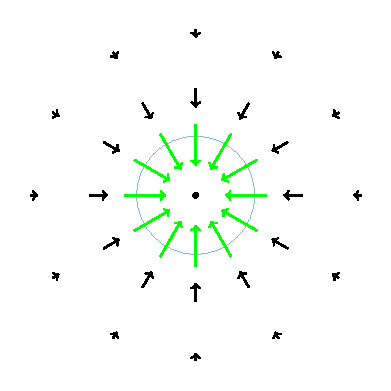
\includegraphics[width=0.8\textwidth,height=\textheight]{figures/grav/fig6.pdf}

}

\caption{Vecteur accélération gravitationnelle en fonction de
l'altitude}

\end{figure}%

Ce mode de représentation porte le nom de \emph{champ gravitationnel}:
on place en chaque point autour de la terre un vecteur dont l'intensité
vaut \(g_h\) et pointant vers le centre de la Terre. Ce mode de
représentation permet d'observer visuellement l'influence que la terre
exerce sur les objets proches d'elle.

Formellement, on définit le champ gravitationnel autour d'un objet comme
suit:

\begin{definition}[]\protect\hypertarget{def-champ}{}\label{def-champ}

Soit un astre de masse \(M\). Le \textbf{champ gravitationnel
\(\overrightarrow{g}_M\)} autour de cet astre est défini en tout point,
d'altitude \(h\), de l'espace comme:

\[
\overrightarrow{g}_M(h) = \frac{k_g M}{(R_M+h)^2} \overrightarrow{u},
\] où \(R_M\) est le rayon de l'astre et \(\overrightarrow{u}\)
représente un vecteur de longueur 1 pointant vers le centre de l'objet
\(M\).

\end{definition}

Le champ gravitationnel permet donc de décrire l'attraction qu'il exerce
sur un objet autour de lui. Plus précisément, tout objet de masse \(m\)
subira une force gravitationnelle décrite par l'équation suivante:

\[
\overrightarrow{F}_{M/m} = m \overrightarrow{g}.
\]

On retrouve bien la loi de la gravitation universelle !

\begin{exercise}[]\protect\hypertarget{exr-champ}{}\label{exr-champ}

Le rayon de la Lune vaut \(1738\text{km}\).

\begin{enumerate}
\def\labelenumi{\arabic{enumi}.}
\tightlist
\item
  Ecris la formule du champ gravitationnel autour de la Lune.
\item
  Peut-on affirmer qu'à la surface de la Lune, le poids d'un astronaute
  est 6 fois plus grand que sur Terre?
\end{enumerate}

\end{exercise}

\section{Orbite géostationnaire et
satellites}\label{orbite-guxe9ostationnaire-et-satellites}

Un satellite géostationnaire est un satellite qui reste immobile par
rapport à la Terre. Cela signifie qu'il doit tourner en
\textbf{exactement 24h}.

\begin{exercise}[]\protect\hypertarget{exr-periode-geo}{}\label{exr-periode-geo}

~

\begin{enumerate}
\def\labelenumi{\arabic{enumi}.}
\tightlist
\item
  Ecris une formule qui lie la période d'un satellite et la force de
  gravitation que celui-ci subit par la Terre.
\item
  Déduis-en l'altitude de ce satellite si celui-ci est en orbite
  géostationnaire.
\end{enumerate}

\end{exercise}




\end{document}
